\documentclass[psamsfonts]{amsart}
\usepackage[utf8]{inputenc}
\usepackage{amsfonts, comment, enumerate}
\usepackage{mathtools}
\usepackage[mathcal]{eucal}
\usepackage[hidelinks]{hyperref}
\hypersetup{
pdftitle={Complexity of deep computations via topology of function spaces}
pdfsubject={Mathematics, Set Theory},
pdfauthor={Luciano Salvetti, Tonatiuh Matos-Wiederhold},
pdfkeywords={}
}
\usepackage{amsmath,amssymb}
\usepackage{xcolor}
\usepackage{amsthm}
\usepackage{pdflscape}
\usepackage{pgfplots}
\usepackage{mathrsfs}
\usepackage{tikz}
\usetikzlibrary{trees}
\usepackage{graphicx}
\graphicspath{ {images/} }
\usepackage{subcaption}

\usepackage[rgb]{xcolor}
\usepackage{pdfcomment}

\newtheorem{thm}{Theorem}[section]
\newtheorem{cor}[thm]{Corollary}
\newtheorem{prop}[thm]{Proposition}
\newtheorem{lem}[thm]{Lemma}
\newtheorem{conj}[thm]{Conjecture}
\newtheorem{quest}[thm]{Question}
\newtheorem*{claim}{Claim}
\newtheorem{fact}[thm]{Fact}
\newtheorem{ppty}[thm]{Property}


\theoremstyle{definition}
\newtheorem{defn}[thm]{Definition}
\newtheorem{question}[thm]{Question}
\newtheorem{defns}[thm]{Definitions}
\newtheorem{con}[thm]{Construction}
\newtheorem{exmp}[thm]{Example}
\newtheorem{exmps}[thm]{Examples}
\newtheorem{notn}[thm]{Notation}
\newtheorem{notns}[thm]{Notations}
\newtheorem{addm}[thm]{Addendum}
\newtheorem{exer}[thm]{Exercise}
\newtheorem{limit}[thm]{Limitation}

\theoremstyle{remark}
\newtheorem{rem}[thm]{Remark}
\newtheorem{rems}[thm]{Remarks}
\newtheorem{warn}[thm]{Warning}
\newtheorem{sch}[thm]{Scholium}

\makeatletter
\let\c@equation\c@thm
\makeatother
\numberwithin{equation}{section}

%\bibliographystyle{plain}

%--------Meta Data: Fill in your info------
\title[Complexity of deep computations via topology of function spaces]{Complexity of deep computations\\ via topology of function spaces}

\author[Dueñez, Iovino, Matos-Wiederhold, Salvetti, Tall]{
Eduardo Dueñez$^{1}$ \qquad
José Iovino$^{1}$ \qquad
Tonatiuh Matos-Wiederhold$^{2}$ \qquad
Luciano Salvetti$^{2}$ \qquad
Franklin D. Tall$^{2}$
}

\usepackage{lineno}
%\linenumbers


\date{\today}
\subjclass[2000]{54H30, 68T27, 68T07, 03C98, 03D15, 05D10}
\keywords{Deep computations, deep equilibrium models, deep learning, physics-informed networks, computational complexity, independence property, NIP,  infinite Ramsey theory,  Baire class~1 functions, Rosenthal compacta, Todorčević trichotomy, Bourgain-Fremlin-Talagrand}

\begin{document}

\maketitle

{\centering\tiny\vspace{-0.6cm}
$^{1}$Department of Mathematics, University of Texas at San Antonio\\
$^{2}$Department of Mathematics, University of Toronto\\
}

\begin{abstract}
We use topological methods to study the complexity of deep computations and limit computations.
We use topology of function spaces, specifically, the classification of Rosenthal compacta, to identify new complexity classes.
We use the language of model theory, specifically,  the concept of  \emph{independence} from Shelah's classification theory, to translate between topology and computation.
We use the theory of Rosenthal compacta to characterize approximability of deep computations, both deterministically and probabilistically.
\end{abstract}

\maketitle

%\setcounter{section}{-1}


\section*{Introduction}


In this paper we study limit behavior of real-valued computations as the values of certain parameters  of the computation model tend towards infinity, or towards zero, or towards some other fixed value, e.g.,  the depth of a neural network tending to infinity, or the time interval between layers of the network tending toward zero.
Recently, particular cases of this situation have attracted considerable attention in deep learning research (e.g., Neural Ordinary Differential Equations~\cite{Chen:2018}, Physics-Informed Neural Networks~\cite{Raissi-Perdikaris-Karniadakis:2019},  and  deep equilibrium models~\cite{Bai:2019}, among others).
In this paper, we combine ideas of topology, measure theory, and  model theory to study these limit phenomena from a unified viewpoint.


Informed by model theory, to each computation in a given computation model, we associate a continuous real-valued function, called the \emph{type} of the computation, that describes the logical properties of this computation with respect to the rest of the model.
This allows us to view computations in any given computational model  as elements of a space of real-valued functions, which is called the \emph{space of types} of the model.
The idea of embedding models of theories into their type spaces is central in model theory.
In the context of this paper, the embedding of computations into spaces of types allows us to utilize the vast theory of topology of function spaces, known as $C_p$-theory, to obtain results about complexity of topological limits of computations.
As we shall indicate next, recent classification results for spaces of functions provide an elegant and powerful machinery to classify computations according to their levels of ``tameness’’ or ``wildness’’, with the former corresponding roughly to polynomial approximability and the latter to exponential approximability.
The viewpoint of spaces of types, which we have borrowed from model theory, thus becomes a ``Rosetta stone’’  that allows us  to interconnect various classification programs: In topology, the classification of Rosenthal compacta pioneered by Todorčević~\cite{Todorcevic_1999_CompactSubsetsBaire}; in logic, the classification of theories developed by Shelah~\cite{Shelah:1990}; and in statistical learning, the notions of PAC learning and VC dimension pioneered by Vapnik and Chervonenkis~\cite{Vapnik-Chervonenkis:1974, Vapnik-Chervonenkis:1971}.



In a previous paper~\cite{alva2024approximability}, we introduced the concept of limits of computations, which we called \emph{ultracomputations} (given they arise as ultrafilter limits of standard computations) and \emph{deep computations}  (following usage in machine learning~\cite{Bai:2019}).
There is a technical difference between both designations, but in this paper, to simplify the nomenclature, we will ignore the difference and use only the term ``deep computation’’.

In \cite{alva2024approximability}, we proved a new ``tame vs wild'' (i.e., polynomial vs exponential) \pdfcomment{I'm not sure that equating ``wild'' with ``exponential'' is actually done in Alva \emph{et al.}} dichotomy for the complexity of deep computations by invoking a classical result of Grothendieck from the 1950s~\cite{Grothendieck:1952}.
Under our model-theoretic Rosetta stone, the property of polynomial approximability of computations is identified with continuous extendibility in the sense of topology, and with the notions of \emph{stability} and \emph{type definability} in model theory.

Simplest among deep computations are those arising as pointwise limits of (continuous) computations proper.
In topology, the \emph{first Baire class}, or \emph{Baire class~1} consists of functions (also called simply ``\emph{Baire-1}'') arising as pointwise limits of  sequences of continuous functions.
Intuitively, the Baire-1 class consists of functions with ``controlled'' discontinuities, and lies just one level of topological complexity away from the Baire class 0 which (by definition) consists of continuous functions.

We prove a new ``tame vs wild'' Ramsey-theoretic dichotomy for complexity of general deep computations by invoking a famous paper by Bourgain, Fremlin and Talagrand from the late 70s~\cite{BFT_1978_PCompactBaire}, and  a new trichotomy for the class of ``tame'' deep computations by invoking an equally celebrated result of Todorčević, from the late 90s, for  functions of the first Baire class~\cite{Todorcevic_1999_CompactSubsetsBaire}.

Todorčević’s trichotomy regards \emph{Rosenthal compacta}; these  are special classes of  topological spaces, defined as compact spaces that can be embedded (homeomorphically identified as a subset) within the space of Baire class~1 functions on some Polish (separable, complete metric) space, under the pointwise convergence topology.
Rosenthal compacta  exhibit  ``topological tameness,'' meaning that they behave in relatively controlled ways;
since the late 70's, they have played a crucial role in understanding the complexity of structures of functional analysis, especially Banach spaces.
Todorčević’s trichotomy has been utilized to settle longstanding problems in topological dynamics and topological entropy~\cite{glasner2022tame}.

Through our Rosetta stone, Rosenthal compacta in topology correspond to the important concept of  ``Non Independence Property'' (known as ``NIP'') in model theory, identified by Shelah~\cite{Shelah:1971,Shelah:1990}, and to the concept of  Probably Approximately Correct learning (known as ``PAC learnability'') in statistical learning theory identified by Valiant~\cite{Valiant:1984}.


Going beyond Todorčević’s trichotomy, we invoke a more recent heptachotomy for Rosenthal compacta obtained by Argyros, Dodos and Kanellopoulos~\cite{argyros2008rosenthal};
they identify seven fundamental ``prototypes" of separable Rosenthal compacta, and  show that any non-metrizable separable Rosenthal compactum must contain a ``canonical'' embedding of one of these prototypes.
They also showed that if a separable Rosenthal compactum is not hereditarily separable, then it must contain an uncountable discrete subspace of the size of the continuum.


We believe that the results presented in this paper show practitioners of computation, or topology, or descriptive set theory, or  model theory, how classification invariants used in their field translate into classification invariants of other fields.
In the interest of accessibility, we do not assume the reader to have previous familiarity with advanced topology, model theory, or computing.
The only technical prerequisites to read this paper are undergraduate-level topology and measure theory.
The necessary topological background beyond undergraduate topology is covered in section~\ref{sec:prelim}.

In section \ref{sec:prelim}, we present basic topological and combinatorial preliminaries, and in section~\ref{S:CCS}, we introduce the structural/model-theoretic viewpoint (no previous exposure to model theory is needed).
Section~\ref{S:Classification} is devoted to the classification of deep computations.

Throughout the paper, our results pertain to classical models of computation (particularly computations involving real-valued quantities that are known and manipulated to a finite degree of precision).
The final Section~\ref{Measure-theoretic NIP} introduces a probabilistic viewpoint, whose development we intend to pursue in future research, extending the present framework to encompass non-deterministic and quantum computations.

\tableofcontents


\section{General topological preliminaries: From continuity\\ to Baire class~1}
\label{sec:prelim}

In this section we present some preliminaries from general topology and function space theory.
We include the proofs of some results for the sake of completeness;
they may be safely skipped by readers familiar with these topics.

Recall that a subset of a topological space is $F_\sigma$ if it is a countable union of closed  sets, and $G_\delta$ if it is a countable intersection of closed sets.
A space is metrizable if its topology agrees with the topology induced by some metric therein.
Two such metrics inducing the same topology may induce quite different properties in the category of metric spaces. 
For example, the interval $(0,1)$ with  the usual metric (as a subset) of the reals is not complete;
however, $(0,1)$ is homeomorphic to the real line, which is complete with respect to the usual metric thereon.
In a metrizable space, every open set is $F_\sigma$; equivalently, every closed set is $G_\delta$.

A \emph{Polish space} is a separable and completely metrizable topological space, i.e., admitting some complete metric inducing its topology.
Although other (possibly incomplete) metrics may induce the same topology, being Polish is a purely topological property.
The most important Polish spaces is the real line~$\mathbb{R}$.
The class of Polish spaces is closed under countable topological products;
in particular, the Cantor space~$2^\mathbb{N}$ (the set of all infinite binary sequences, endowed with the product topology), the Baire space $\mathbb{N}^\mathbb{N}$ (the set of all infinite sequences of naturals, also with the product topology), and the space $\mathbb{R}^\mathbb{N}$ of sequences of real numbers are all Polish.

The following result is a cornerstone of descriptive set theory, closely tied to the work of Wacław Sierpiński and Kazimierz Kuratowski, with proofs often built upon their foundations and formalized later, notably involving Stefan Mazurkiewicz's work on complete metric spaces.

\begin{fact}
A subset \(A\) of a Polish space \(X\) is itself Polish in the subspace topology if and only if it is a  $G_{\delta }$ set.
In particular, closed subsets and open subsets of Polish spaces are also Polish spaces.
\end{fact}

Given two topological spaces $X$ and $Y$ we denote by $C_p(X,Y)$ the set of all continuous functions $f:X\rightarrow Y$ endowed with the topology of pointwise convergence.
The space $C_p(X, \mathbb{R})$ of continuous real functions on~$X$ is denoted simply~$C_p(X)$.
A natural question is, how do topological properties of $X$ translate into $C_p(X)$ and vice versa?
This general question, and the study of these spaces in general, is the concern of $C_p$-theory, an active field of research in general topology which was pioneered by A.~V.~Arhangel’skiĭ and his students in the 1970's and 1980's~\cite{Arkhangelskii:1992}.
This field has found many applications in model theory and functional analysis.
For a recent survey, see~\cite{tkachuk2011cp}.
 
 A  \emph{Baire class~1} function between topological spaces is a function that can be expressed as the pointwise limit of a sequence of continuous functions.
If $X$ and $Y$ are topological spaces, the space of Baire class~1 functions $f:X\rightarrow Y$ endowed with the topology of pointwise convergence is denoted $B_1(X,Y)$ (as above, $B_1(X, \mathbb{R})$ is denoted $B_1(X)$).
Clearly, $C_p(X,Y)\subseteq B_1(X,Y)$.
The Baire hierarchy of functions was introduced by René-Louis Baire in his 1899 doctoral thesis, \emph{Sur les fonctions de variables réelles}.
His work moved away from the 19th-century preoccupation with ``pathological'' functions toward a constructive classification based on pointwise limits.

A topological space $X$ is \emph{perfectly normal} if it is normal and every closed subset of $X$ is a $G_\delta$ (equivalently, every open subset of $X$ is a $F_\sigma$).
Every metrizable space (hence, every Polish space) is perfectly normal.

A topological space $X$ is \emph{Baire} if every countable intersection of dense open sets is non-empty.
The Baire Category Theorem states that every completely metrizable space (hence, every Polish space) is Baire in the sense above.

The following fact was established by Baire in his 1899 thesis.
A proof can be found in~\cite[Section 10]{Todorcevic_1997_TopicsTop}.

\begin{fact}[Baire]\label{baire}
    If $X$ is perfectly normal, then the following conditions are equivalent for a function $f:X\to \mathbb{R}$:
    \begin{itemize}
        \item[(1)] $f$ is a Baire class~1 function, that is,  $f$ is a pointwise limit of continuous functions.
        \item[(2)] $f^{-1}[U]$ is an $F_\sigma$ subset of $X$ whenever $U\subseteq Y$ is open.
    \end{itemize}
    If $X$ is Baire, then (1) and (2) are equivalent to:
    \begin{itemize}
        \item[(3)] For every closed $F\subseteq X$, the restriction $f|_F$ has a point of continuity.
    \end{itemize}
    Moreover, if $X$ is Polish and $f\notin B_1(X)$, then there exist countable $D_0,D_1\subseteq X$ and reals $a<b$ such that
    \[
    D_0\subseteq f^{-1}(-\infty,a],
    \quad
    D_1\subseteq f^{-1}[b,\infty),
    \quad
    \overline{D_0}=\overline{D_1}.
    \]
\end{fact}

A subset $L$ of a topological space $X$ is \emph{relatively compact} in $X$ if the closure of $L$ in $X$ is compact.
Relatively compact subsets of $B_1(X)$ (for $X$ Polish) have been objects of interest  for researchers in Analysis and Topological Dynamics.
We begin with the following well-known result.
Recall that a set $A\subseteq\mathbb{R}^X$ of real-valued functions is \emph{pointwise bounded} if for every $x\in X$ there is $M_x \ge 0$ (a \emph{pointwise bound at~$x$}) such that $|f(x)| \le M_x$ for all $f\in A$.
We include a proof for the reader's convenience:

\begin{lem}
    Let $X$ be a Polish space and $A\subseteq B_1(X)$ be pointwise bounded.
The following are equivalent:
    \begin{enumerate}[(i)]
        \item
        $A$ is relatively compact in $B_1(X)$.
        \item
        $A$ is relatively countably compact in $B_1(X)$, i.e., every countable subset of $A$ has an accumulation point in $B_1(X)$.
        \item
        $\overline{A}\subseteq B_1(X)$, where $\overline{A}$ denotes the closure in $\mathbb{R}^X$.
    \end{enumerate}
\end{lem}

\begin{proof}
    (i)$\Rightarrow$(ii) Relative compact subsets of any space are countably compact therein.


    (ii)$\Rightarrow$(iii)
Consider any $f\in\overline A$ and any countable subset $\{x_i\}_{i\in \mathbb{N}}\subseteq X$.
We claim that there is a sequence $\{f_n\}_{n\in\mathbb{N}}\subseteq A$ such that $\lim_{n\to\infty}f_n(x_i)=f(x_i)$ for all $i\in \mathbb{N}$.
Since $A$ carries the relative product topology, for each $n\in \mathbb{N}$ there exists $f_n\in A$ such that $|f_n(x_i) - f(x_i)| < \frac{1}{n}$ for all $i \le n$;
the sequence $\{f_n\}$ is as claimed.
Seeking a contradiction, assume that $A$ is relatively countably compact in~$B_1(X)$, but there exists some $f\in \overline{A}\setminus B_1(X)$.
    By Fact \ref{baire}, there are countable $D_0,D_1\subseteq X$ with $\overline {D_0}=\overline{D_1}$, and $a<b$ such that $D_0\subseteq f^{-1}(-\infty,a]$ and $D_1\subseteq f^{-1}[b,\infty)$.
Per the claim above, let $\{f_n\}_{n\in\mathbb{N}}\subseteq A$ satisfy $\lim_{n\to\infty}f_n(x)=f(x)$ for all $x\in D_0\cup D_1$ (the latter being a countable set).
By relative countable compactness of~$A$, there is an accumulation point $g\in B_1(X)$ of $\{f_n\}_{n\in\mathbb{N}}$;
clearly, $f$ and $g$ agree on $D_0\cup D_1$.
Thus $g$ takes values $g(x_i) = f(x_i) \le  a$ as well as values $g(x_j) = f(x_j) \ge b > a$ on any open subset of the closed set $\overline{D_0} = \overline{D_1}$, contradicting the implication (1)$\Rightarrow$(3) in Fact~\ref{baire}.

(iii)$\Rightarrow$(i)   For each $x\in X$, let $M_x \ge 0$ be a pointwise bound for~$A$ thereat.
Being necessarily a closed subset of the compact space (being product of compacta) $\prod_{x\in X}[-M_x,M_x] \subseteq \mathbb{R}^X$,  it follows that $\overline{A}$ is compact;
by~(iii), it is also the closure of~$A$ in $B_1(X)$ \emph{a fortiori}.
Thus, $A$ is relatively compact in $B_1(X)$.
\end{proof}

\subsection{From Rosenthal's dichotomy to the Bourgain-Fremlin-Talagrand dichotomy to Shelah's NIP}

In metrizable spaces, points of the closure of some subset can always be approximated by points in the set proper, via a convergent sequence.
For more complicated spaces, such as $C_p$-spaces, this fails in remarkable ways.
The $n$-th coordinate map $p_n: 2^{\mathbb{N}}\to\{0,1\}$ on the Cantor space $X = 2^\mathbb{N}$ ($= \{0, 1\}^{\mathbb{N}}$) is continuous for each $n\in \mathbb{N}$, and one can show (e.g., \cite[Chapter~1.1]{Todorcevic_1997_TopicsTop}) that $\{p_n\}_{n\in\mathbb{N}}$ is closed, but has \emph{no} convergent subsequences, in $Y = C_p(X)$:
in a sense, such example exhibits the worst failure of sequential convergence possible.
The closure of $\{p_n\}$ in $\{0, 1\}^X$ (or in $\mathbb{R}^{X}$ for that matter) realizes the \emph{Stone-Čech compactification $\beta\mathbb{N}$} of the discrete space of natural numbers;
it is an important object of study in general topology.

The following theorem, proved by Haskell Rosenthal in 1974, is fundamental in functional analysis and captures a sharp division in the behavior of sequences in a Banach spaces.

\begin{thm}[Rosenthal's Dichotomy, \cite{Rosenthal:1974}]
\label{T:Rosenthal}
    If $X$ is Polish and $\{f_n\}\subseteq C_p(X)$ is pointwise bounded, then $\{f_n\}_{n\in\mathbb{N}}$ has a convergent subsequence, or a subsequence whose closure in $\mathbb{R}^X$ is homeomorphic to~$\beta\mathbb{N}$.
\end{thm}

In other words, a pointwise bounded set of continuous functions contains either a convergent subsequence, or a subsequence whose closure is essentially the same as the example mentioned in the previous paragraphs (i.e., ``wildest'' possible).

The genesis of Theorem~\ref{T:Rosenthal} was Rosenthal's ``$\ell_1$-Theorem'', which states that a Banach space includes an isomorphic copy of $\ell_1$  (the space of absolutely summable sequences), or else every bounded sequence therein is weakly Cauchy.
The $\ell_1$-Theorem connects diverse areas:
Banach space geometry, Ramsey theory, set theory, and topology of function spaces.

As we move from $C_p(X)$ to the larger space $B_1(X)$, a dichotomy paralleling the $\ell_1$-Theorem holds:
Either every point of the closure of a set of functions is a Baire class-1 function, or there is a sequence in the set behaving in the wildest possible way.
Such theorem is usually not phrased as a dichotomy, but rather as an equivalence as in Theorem~\ref{BFT} below.

First, we introduce some useful notation.
For any set $A\subseteq \mathbb{R}^X$ and any real $a$, define
\begin{align*}
  X^A_{\le a} &\coloneqq \bigcap_{f\in A}f^{-1}(-\infty,a] = \{x\in X: \text{$f(x)\le a$ for all $f\in A$}\},\\
  X^A_{\ge a} &\coloneqq \bigcap_{f\in A}f^{-1}[a, +\infty) = \{x\in X: \text{$f(x)\ge a$ for all $f\in A$}\}.
\end{align*}
(In case $A=\emptyset$, we define $X^\emptyset_{\ge a} = X = X^\emptyset_{\le a}$.)
For any sequence $\{f_n\}\subseteq \mathbb{R}^X$ and $I\subseteq \mathbf{N}$, define $I^{\complement} \coloneqq \mathbb{N}\setminus I$ and $f_I \coloneqq \{f_i: i\in I\}$.

\begin{thm}[``The BFT Dichotomy''. Bourgain-Fremlin-Talagrand {\cite{BFT_1978_PCompactBaire}}]
\label{BFT}
    Let $X$ be a Polish space and $A\subseteq C_p(X)$ be pointwise bounded.
The following are equivalent:
    \begin{enumerate}[(i)]
        \item $A$ is relatively compact in $B_1(X)$.
        \item For every $\{f_n\}_{n\in\mathbb{N}}\subseteq A$ and every $a<b$ there is $I\subseteq\mathbb{N}$ such that $X_{\le a}^{f_I} \cap X_{\ge b}^{f_{I^{\complement}}} = \emptyset$.
    \end{enumerate}
\end{thm}
(As stated above, the BFT Dichotomy is a particular case of the equivalence (iv)$\Leftrightarrow$(viii) in {\cite[Theorem 4D]{BFT_1978_PCompactBaire}}:
on a Polish space, a real function is Baire-1 iff it is $K$-analytic.)

The sets $X_{\le a}^{f_I}$ and $X_{\ge b}^{f_{I^{\complement}}}$ appearing in condition Theorem~\ref{BFT}\emph{(ii)} are defined, respectively, in terms of $|I|$-many inequalities of the form $f_i(x)\le a$, and $|I^{\complement}|$-many of the form $f_j(x)\ge b$.
Thus, at least one of  $X_{\le a}^{f_I}$ and $X_{\ge b}^{f_{I^{\complement}}}$ is defined by the satisfaction of infinitely (countably) many inequalities.
For our purposes, it is more natural to consider only finitely many inequalities at a time, which motivates the definitions below.

\begin{defn}\label{def:NIP-fns}
    We say that \emph{$A$ has the No-Independence Property (NIP)} if, for all sequences $\{f_n\}_{n\in\mathbb{N}}\subseteq A$ and reals $a<b$ there exist finite disjoint sets $E,F\subseteq\mathbb{N}$ such that $X_{\le a}^{f_E} \cap X_{\ge b}^{f_F} = \emptyset$.
    We say that such $E, F$ \emph{witness NIP for $A$, $\{f_n\}$ and $a, b$}.
    For emphasis, we say that NIP in this sense is \emph{finitary} NIP.

    A set $A\subseteq \mathbb{R}^X$ \emph{has the Independence Property (IP)} if it does not have NIP, i.e., there exists a sequence $\{f_n\}_{n\in\mathbb{N}}\subseteq A$ and reals $a<b$ such that for every pair of finite disjoint sets $E,F\subseteq\mathbb{N}$, we have $X_{\le a}^{f_E} \cap X_{\ge b}^{f_F} \ne \emptyset$.
    Again, such IP will be called \emph{finitary} for emphasis.
\end{defn}

If the word ``finite'' is omitted in the above definitions, we obtain the definitions of \emph{countable} NIP (weaker than finitary NIP) and \emph{countable} IP (stronger than finitary IP), respectively.


If we insist on witnesses $E,F\subseteq \mathbf{N}$ such that $E\cup F = \mathbf{N}$, we call the respective properties ``BFT-NIP'' (even weaker than countable NIP) and ``BFT-IP'' (even stronger than countable IP).
Evidently, the condition in Theorem~\ref{BFT}\emph{(ii)} is simply that $A$ has BFT-NIP.

\begin{prop}\label{prop:BFT-finitary-cpct}
  If $X$ is compact and $A\subseteq C_p(X)$, then $A$ has BFT-NIP if and only if it has finitary NIP.
\end{prop}
\begin{proof}
  Trivially (as per the preceding discussion), finitary NIP implies BFT-NIP.
  Reciprocally, assume that $X$ is compact and has finitary IP.  
  Fix $A\subseteq C_p(X)$, a sequence $\{f_n\}\subseteq A$ and reals $r<s$.
  For any $I, J\subseteq \mathbb{N}$ (eventually disjoint in applications), write $X_{I,J}$ for $X^{f_I}_{\le r}\cap X^{f_J}_{\ge s}$.
  For $I\subseteq I'\subseteq \mathbb{N}$ and $J\subseteq J'\subseteq \mathbb{N}$, we have $X_{I,J}\supseteq X_{I',J'}$;
  moreover, $X_{I,J} = \bigcap_{E\subseteq I, F\subseteq J} X_{E, F}$, where the index variables $E\subseteq I$, $F\subseteq J$ range over \emph{finite} subsets of~$I, J$, respectively.
  Clearly, $E, F\subseteq \mathbb{N}$ witness finitary NIP for $\{f_n\}$ iff $X^{E,F}=\emptyset$.

  Fix $I\subseteq \mathbb{N}$.
  Since $\{f_n\}\subseteq A\subseteq C_p(X)$ is a sequence of continuous functions, and $X$ is compact, the nested family $\{X_{E,F}: E\subseteq I, F\subseteq I^{\complement}\}$ consists of closed, thus compact, sets.
  Since $A$ has finitary IP by hypothesis, the nested family consists of nonempty sets, hence its intersection $X_{I,I^{\complement}}\ne\emptyset$ by compactness.
  This holds for arbitrary $\{f_n\}\subseteq A$ and $r<s$, so $A$ has BFT-IP.
\end{proof}

Henceforth, by IP/NIP we will mean \emph{finitary} IP/NIP unless otherwise specified.

\begin{thm}
\label{BFT2}
    Let $X$ be a compact Polish space.
Then, for every pointwise bounded  $A\subseteq C_p(X)$, one and exactly one of the following two conditions must hold:
        \begin{enumerate}[(i)]
        \item $\overline{A}\subseteq B_1(X)$.
        \item $A$ has IP.
    \end{enumerate}
\end{thm}
\begin{proof}
  Corollary of Theorem~\ref{BFT} and Proposition~\ref{prop:BFT-finitary-cpct}.
\end{proof}


The Independence Property was first isolated by Saharon Shelah in model theory as a dividing line between theories whose models are ``tame'' (corresponding to NIP) and theories whose models are ``wild" (corresponding to IP).
See~\cite[Definition 4.1]{Shelah:1971}, \cite{Shelah:1990}.
We will discuss this dividing line in more detail in the next section.


\subsection{NIP as a universal dividing line between polynomial and exponential complexity}

The particular case of the BFT dichotomy (Theorem~\ref{BFT}) when $A$ consists of $\{0,1\}$-valued (i.e., $\{\text{Yes},\text{No}\}$-valued) strings was discovered independently, around 1971-1972 in many foundational contexts related to polynomial (``tame") vs exponential (``wild'') complexity:  In model theory, by Saharon Shelah~\cite{Shelah:1971}, \cite{Shelah:1990}, in  combinatorics, by Norbert Sauer~\cite{Sauer:1972}, and Shelah~\cite{Shelah:1972}, \cite{Shelah:1990}, and in statistical learning, by Vladimir Vapnik and Alexey Chervonenkis~\cite{Vapnik-Chervonenkis:1971}, \cite{Vapnik-Chervonenkis:1974}.


\begin{description}

\item[In model theory]
Shelah's classification theory is a foundational program in mathematical logic devised to categorize first-order theories based on the complexity and structure of their models.
A theory $T$ is considered classifiable in Shelah's sense if the number of non-isomorphic models of $T$ of a given cardinality can be described by a bounded number of numerical invariants.
In contrast, a theory $T$ is unclassifiable if the number of models of $T$ of a given cardinality is the maximum possible number.
A key fact is that the  number of models of $T$ is directly impacted by the number of  \emph{types} over  sets of parameters in models of $T$; a controlled number of types is a characteristic of a classifiable theory.


In Shelah's classification program~\cite{Shelah:1990}, theories without the independence property (called NIP theories, or dependent theories) have a well-behaved, ``tame" structure; the number of types over a set of parameters of size $\kappa$ of such a theory is of polynomially or similar ``slow" growth on $\kappa$.

In contrast, theories with the Independence Property  (called IP theories) are considered ``intractable" or ``wild''.
A theory with the Independence Property produces the maximum possible number of types over a set of parameters;  for a set of parameters of cardinality $\kappa$, the theory will have $2^{2^{\kappa}}$-many distinct types.

 \item[In combinatorics]
   Sauer~\cite{Sauer:1972} and Shelah~\cite{Shelah:1972} proved the following independently:
   Let $\mathscr{F}$ be a family of subsets of some set $S$.
   Either:
   for every $n\in\mathbb{N}$ there is  a set $A\subseteq S$ with $|A|=n$ such that $|\{S_i\cap A: i\in\mathbb{N}\}|=2^n$ ($\mathscr{F}$ has ``exponential complexity'');
or: there exists $N\in\mathbb{N}$ such that  for every $A\subseteq S$ with $|A|\ge N$, one has
\[
|\{S_i\cap A: i\in\mathbb{N}\}| \le \sum_{i=0}^{N-1} \binom{|A|}{i}.
\]
($\mathscr{F}$ has ``polynomial complexity'').
Clearly, any family $\mathscr{F}$ of subsets of a \emph{finite} set $S$ has polynomial complexity.
The ``polynomial'' name is justified:
indeed, for fixed $N>0$, as a function of the size $|A| = m > 0$, we have
\begin{equation*}
  \sum_{i=0}^{N-1} \binom{m}{i}
  \le \sum_{i=0}^{N-1}\frac{m^{i}}{i!}
  \le \left( \sum_{i=0}^{N-1}\frac{1}{i!} \right)\cdot m^{N-1}\cdot
  < e\cdot m^{N-1} = O \left( m^N \right).
\end{equation*}
(More precisely, the order of magnitude is $O(m^{N-1})$:
polynomial in $m$ for $N$ fixed.)

 \item[In machine learning]
Readers familiar with statistical learning may recognize the Sauer-Shelah lemma as the dichotomy discovered and proved slightly  earlier (1971) by Vapnik and Chervonenkis~\cite{Vapnik-Chervonenkis:1971, Vapnik-Chervonenkis:1974} to address the problem of uniform convergence in statistics.
The least integer $N$ given by the preceding paragraph, when it exists, is called the \emph{VC-dimension} of $\mathscr{F}$;
it is a core concept in machine learning.
If such an integer $N$ does not exist, we say that the VC-dimension of $\mathscr{F}$ is infinite.
The lemma provides upper bounds on the number of data points (sample size) needed to learn a concept class of known VC dimension~$d$ up to a given admissible error in the statistical sense.
The Fundamental Theorem of Statistical Learning states that a hypothesis class is PAC-learnable (PAC stands for ``Probably Approximately Correct'') if and only if its VC dimension is finite.
 
\end{description}
 
\subsection{Rosenthal compacta}
 
 The universal classification implied by Theorem~\ref{BFT}, as attested by the examples outlined in the preceding section, led to the following definition (by Gilles Godefroy~\cite{Godefroy:1980}):

\begin{defn}
\label{D:Rosenthal compacta}
A Rosenthal compactum is any topological space realized as a compact subset of the space $B_1(X) = B_1(X, \mathbb{R})$ (equipped with the topology of pointwise convergence) of all real functions of the first Baire class on some Polish space~\(X\).
\end{defn}
A Rosenthal compactum~$K$ is necessarily Hausdorff since it is a topological subspace of the Hausdorff product space $\mathbb{R}^X$.

Rosenthal compacta possess significant topological and dynamical tameness properties.
They play an important role in functional analysis,  measure theory, dynamical systems, descriptive set theory, and model theory;
in this paper, we use them to study deep computations.
For this, we shall first focus on countable languages, which is the theme of the next subsection.


\subsection{The special case $B_1(X,\mathbb{R}^\mathcal{P})$   with $\mathcal{P}$ countable.}

Fix an arbitrary (at most) countable set~$\mathcal{P}$ whose elements $P\in \mathcal{P}$ will be called \emph{predicate symbols} or \emph{formal predicates}.
Our present goal is to characterize relatively compact subsets of $B_1(X,\mathbb{R}^\mathcal{P})$.
For $P\in\mathcal{P}$, let $\pi_P:\mathbb{R}^\mathcal{P}\rightarrow\mathbb{R}$ be the corresponding projection (``$P$-th coordinate'' map).
The next lemma reduces the study of (Baire-1) functions into~$\mathbb{R}^{\mathcal{P}}$ to the special case of real-valued ones.

%In fact, $\mathbb{R}$ and any other Polish space is embeddable as a closed subspace of $\mathbb{R}^\mathcal{P}$.

\begin{lem}\label{baire 1 and projections}
    Let $X$ be a Polish space and let $\mathcal{P}$ be any (at most) countable set.
    For all $f: X\to \mathbb{R}$, the equivalence $f\in B_1(X,\mathbb{R}^\mathcal{P})$ if (and only if) $\pi_P\circ f\in B_1(X)$ for all $P\in\mathcal{P}$ holds.
\end{lem}
\begin{proof}
  Any open $U\subseteq \mathbb{R}^{\mathcal{P}}$ is a union of basic open sets each a finite intersection of sets of the form $\tilde{U} = \pi_P^{-1}[V]$ where $V\subseteq \mathbb{R}$ is open and $P\in\mathcal{P}$.
  It suffices to let $V$ vary over the (countable set) of open intervals with rational endpoints.
  Such $V$ are $F_{\sigma}$ in~$\mathbb{R}$.
  Since the intersection of finitely many $F_{\sigma}$ is still $F_{\sigma}$, the correspondingly obtained basis of~$\mathbb{R}^{\mathcal{P}}$ consists of $F_{\sigma}$ (open) sets, and is countable as well
  (in particular, $\mathbb{R}^{\mathcal{P}}$ is second countable for $\mathcal{P}$ countable);
  it follows that all open $U\subseteq \mathbb{R}^{\mathcal{P}}$ are $F_{\sigma}$.

  Beginning the proof proper, suppose that $\pi_P\circ f\in B_1(X)$ for all $P\in\mathcal{P}$.
  By the equivalence (1)$\Leftrightarrow$(2) in Fact~\ref{baire}, it suffices to show that $f^{-1}[U]$ is $F_{\sigma}$ for all open $U\subseteq \mathbb{R}^{\mathcal{P}}$;
  indeed, by the argument above, it suffices to consider subbasics $U = \pi_P[V]$ with $V$ open and $P\in \mathcal{P}$.
  All functions $\pi_P\circ f$ are Baire~1 by hypothesis, so $f^{-1}[U] = (\pi_P\circ f)^{-1}[V]$ is $F_{\sigma}$;
  therefore, $f$ is itself Baire~1.

  The converse is obvious.
\end{proof}




Below we consider $\mathcal{P}$ with the discrete topology.
For each $f:X\rightarrow\mathbb{R}^\mathcal{P}$ denote $\hat f(P,x):=\pi_P\circ f(x)$ for all $(P,x)\in\mathcal{P}\times X$.
Similarly, for each $g:\mathcal{P}\times X\rightarrow\mathbb{R}$ denote $\check g(x)(P):=g(P,x)$.
Given $A\subseteq (\mathbb{R}^\mathcal{P})^X$, we denote $\hat A$ as the set of all $\hat f$ such that $f\in A$.
Note that the map $\left(\mathbb{R}^\mathcal{P}\right)^X\to\mathbb{R}^{\mathcal{P}\times X}$ given by $f\mapsto\hat f$ is a homeomorphism and its inverse is given by $g\mapsto\check g$.

\begin{lem}\label{homeo}
    Let $X$ be a Polish space and $\mathcal{P}$ be countable.
Then, $f\in B_1(X,\mathbb{R}^\mathcal{P})$ if and only if $\hat f\in B_1(\mathcal{P}\times X)$.
\end{lem}

\begin{proof}
    ($\Rightarrow$) By Lemma~\ref{baire 1 and projections}, given an open set of reals $U$, we have  $f^{-1}[\pi_P^{-1}[U]]$ is $F_\sigma$ for every $P\in\mathcal{P}$.
Given that $\mathcal{P}$ is a discrete countable space, we observe that
    $$\hat f^{-1}[U]=\bigcup_{P\in\mathcal{P}}\left(\{P\}\times f^{-1}[\pi_P^{-1}[U]]\right)
    $$ is an $F_\sigma$ as well.
    
    ($\Leftarrow$) By lemma \ref{baire 1 and projections} it suffices to show that $\pi_P\circ f\in B_1(X)$ for all $P\in\mathcal{P}$.
Fix an open $U\subseteq\mathbb{R}$.
Write $\hat{f}^{-1}[U]=\bigcup_{n\in\mathbb{N}}F_n$ where $F_n$ is closed in $\mathcal{P}\times X$.
Then,
    $$(\pi_P\circ f)^{-1}[U]=\bigcup_{n\in\mathbb{N}}\{x\in X:(P,x)\in F_n\}$$
    which is $F_\sigma$.
\end{proof}

Given $A\subseteq Y^X$ and $K\subseteq X$ we write $A|_K:=\{f|_K:f\in A\}$, i.e., the set of all restrictions of functions in $A$ to $K$.
The following Theorem is a slightly more general version of Theorem \ref{BFT}.

\begin{thm}\label{Generalized BFT}
    Assume that $\mathcal{P}$ is countable, $X$ is a Polish space, and $A\subseteq C_p(X,\mathbb{R}^\mathcal{P})$ is such that $\pi_P\circ A$ is pointwise bounded for all $P\in\mathcal{P}$.
The following are equivalent for every compact $K\subseteq X$:

    \begin{enumerate}[(i)]
        \item $\overline{A|_K}\subseteq B_1(K,\mathbb{R}^\mathcal{P})$.
        \item $\pi_P\circ A|_K$ satisfies the NIP for every $P\in\mathcal{P}$.
    \end{enumerate}
\end{thm}

\begin{proof}
    (i)$\Rightarrow$(ii).
Let $P\in\mathcal{P}$.
Fix $\{f_n\}_{n\in\mathbb{N}}\subseteq A$ and $a<b$.
By (i), we have $\overline{A|_K}\subseteq B_1(K,\mathbb{R}^\mathcal{P})$.
Applying the homeomorphism $f\mapsto \hat{f}$ and using lemma \ref{homeo} we get $\overline{\hat{A}|_{\mathcal{P}\times K}}\subseteq B_1(\mathcal{P}\times K)$.
By Theorem \ref{BFT}, there is $I\subseteq\mathbb{N}$ such that
    $$(\mathcal{P}\times K)\cap\bigcap_{n\in I}\hat{f_n}^{-1}(-\infty,a]\cap\bigcap_{n\notin I}\hat{f_n}^{-1}[b,\infty)=\emptyset$$
    Hence,
    $$K\cap\bigcap_{n\in I}(\pi_P\circ f_n)^{-1}(-\infty,a]\cap\bigcap_{n\notin I}(\pi_P\circ f_n)^{-1}[b,\infty)=\emptyset$$
    By the compactness of $K$, there are finite $E\subseteq I$ and $F\subseteq\mathbb{N}\backslash I$ such that
    $$K\cap\bigcap_{n\in E}(\pi_P\circ f_n)^{-1}(-\infty,a]\cap\bigcap_{n\in F}(\pi_P\circ f_n)^{-1}[b,\infty)=\emptyset$$
    Thus, $\pi_P\circ A|_L$ satisfies the NIP.

    (ii)$\Rightarrow$(i) Fix $f\in\overline{A|_K}$.
By lemma \ref{baire 1 and projections} it suffices to show that $\pi_P\circ f\in B_1(K)$ for all $P\in\mathcal{P}$.
By (ii), $\pi_P\circ A|_K$ satisfies the NIP.
Hence, by Theorem \ref{BFT} we have $\overline{\pi_P\circ A|_K}\subseteq B_1(K)$.
But then, $\pi_P\circ f\in\overline{\pi_P\circ A|_K}\subseteq B_1(K)$.
\end{proof}

Lastly, a simple but useful lemma that helps understand when we restrict a set of functions to a specific subspace of the domain space, we may always assume that the subspace is closed, as replacing the subspace by its closure has no effect on NIP.

\begin{lem}\label{NIP and closure}
    Assume that $X$ is Hausdorff and that $A\subseteq C_p(X)$.
The following are equivalent for every $L\subseteq X$:
    \begin{enumerate}[(i)]
        \item
        $A_L$ satisfies the NIP.
        \item
        $A|_{\overline{L}}$ satisfies the NIP.
    \end{enumerate}
\end{lem}

\begin{proof}
    It suffices to show that (i)$\Rightarrow$(ii).
Suppose that (ii) does not hold, i.e., that there are $\{f_n\}_{n\in\mathbb{N}}\subseteq A$ and $a<b$ such that for all finite disjoint $E,F\subseteq\mathbb{N}$:
    $$\overline{L}\cap\bigcap_{n\in E}f_n^{-1}(-\infty,a]\cap\bigcap_{n\in F}f_n^{-1}[b,\infty)\neq\emptyset.$$
    Pick $a'<b'$ such that $a<a'<b'<b$.
Then, for any finite disjoint $E,F\subseteq\mathbb{N}$ we can choose
    $$x\in\overline{L}\cap\bigcap_{n\in E}f_n^{-1}(-\infty,a')\cap\bigcap_{n\in F}f_n^{-1}(b',\infty)$$
    By definition of closure:
    $$L\cap\bigcap_{n\in E}f_n^{-1}(-\infty,a']\cap\bigcap_{n\in F}f_n^{-1}[b',\infty)\neq\emptyset.$$
    This contradicts (i).
\end{proof}

\section{Compositional computation structures: A structural approach \\ to floating-point computation}
\label{S:CCS}


In this section, we connect function spaces with floating point computation.
We start by summarizing some basic concepts from \cite{alva2024approximability}.

A \emph{computation states structure} is a pair $(L,\mathcal{P})$, where $L$ is a set whose elements we call \emph{states} and $\mathcal{P}$ is a collection of real-valued functions on $L$ that we call \emph{predicates}.
For a state $v\in L$, the  \emph{type} of $v$ is defined as  the indexed family
\[
\operatorname{tp}(v)= (P(v))_{P\in \mathcal{P}}\in\mathbb{R}^\mathcal{P}.
\]
For each $P\in \mathcal{P}$, we call the value $P(v)$ the $P$-th \emph{feature} of~$v$.
A \emph{transition} of a computation states structure  $(L,\mathcal{P})$ is a map $f:L\to L$.


Intuitively, $L$ is the set of states of a computation,  and the predicates  $P \in\mathcal{P}$ are primitives that are given and accepted as computable.
We think of  each state $v\in L$ as being uniquely characterized by its type $\operatorname{tp}(v)$.
Thus,  in practice, we identify $L$ with a subset of $\mathbb{R}^\mathcal{P}$.
A typical case will be when $L=\mathbb{R}^\mathbb{N}$ or $L=\mathbb{R}^n$ for some positive integer $n$ and there is a predicate $P_i(v) = v_i$ for each of the coordinates $v_i$ of~$v$.
We regard the space of types as a topological space, endowed with the topology of pointwise convergence inherited from $\mathbb{R}^\mathcal{P}$.
In particular, for each $P\in \mathcal{P}$, the projection map $v\mapsto P(v)$ is continuous.


\begin{defn}
Given a computation states structure $(L,\mathcal{P})$, any element of $\mathbb{R}^\mathcal{P}$  in the image of $L$ under the map $v\mapsto \operatorname{tp}(v)$ will be called a \emph{realized type}.
The topological closure of the set of realized types in $\mathbb{R}^\mathcal{P}$ (endowed with the pointwise convergence topology) will be called the \emph{space of types} of  $(L,\mathcal{P})$, denoted $\mathcal{L}$.
Elements of $\mathcal{L}\setminus L$ will be called \emph{unrealized types}.
\end{defn}

In  traditional, compact-valued, model theory, the space of types of a structure is viewed as a sort of compactification of the structure, and the compactness of type spaces plays a central role.
However, here we are dealing with real-valued structures, and the space  $\mathcal{L}$ defined above is not necessarily compact.
To bypass this obstacle, we follow the idea introduced in~\cite{alva2024approximability} of covering $\mathcal{L}$ by ``thin'' compact subspaces that we call \emph{shards}.
The formal definition of shard is next.

\begin{defn}
A \emph{sizer} is a tuple $r_{\bullet}=(r_P)_{P\in\mathcal{P}}$ of positive real numbers indexed by $\mathcal{P}$.
Given a sizer $r_\bullet$, we define the $r_\bullet$-\emph{shard} as:
\[
L[r_\bullet]=L\cap\prod_{P\in\mathcal{P}}[-r_P,r_P].
\]

For a sizer  $r_{\bullet}$, the \emph{$r_{\bullet}$-type shard} is defined as $\mathcal{L}[r_\bullet]=\overline{L[r_\bullet]}$.

%A collection $R$ of sizers is called \emph{exhaustive} if $\mathcal{L}_{\text{sh}}=\bigcup_{r_{\bullet}\in R}\mathcal{L}[r_\bullet]$.
We define $\mathcal{L}_{\text{sh}}$, as the union of all type-shards.

\end{defn}

%\begin{rem}
%Even though our type space $\mathcal{L}$ is not compact, the fact that it can be covered by shards gives us two advantages:
%\begin{enumerate}[(i)]
%\item
%It gives us access to the rich theory of Lindel\"of-$\Sigma$ spaces and $K$-analytic spaces
%\item
%Families of functions in a given shard are pointwise bounded, which gives us access to the Bourgain-Fremlin-Talagrand dichotomy (Theorem~\ref{BFT}, \ref{BFT-2F} and the theory of Rosenthal compacta.
%\end{enumerate}
%\end{rem}

\subsection{Compositional Computation Structures} 

\begin{defn}
\label{D:CCS}
A \emph{Compositional Computation Structure} (CCS) is a triple $(L,\mathcal{P},\Gamma)$, where
\begin{itemize}
\item
 $(L,\mathcal{P})$ is a computation states structure, and
 \item
 $\Gamma\subseteq L^L$ is a semigroup under composition.
\end{itemize}

The elements of the  semigroup $\Gamma$ are called the \emph{computations} of the structure $(L,\mathcal{P},\Gamma)$.

If $\Delta\subseteq\Gamma$, we say that $\Delta\subseteq\Gamma$ is \emph{$R$-confined} if $\gamma|_{L[r_\bullet]}:L[r_\bullet]\to L[r_\bullet]$ for every $r_\bullet\in R$ and $\gamma\in \Delta$.
Elements in $\overline{\Gamma}\subseteq \mathcal{L}_{\text{sh}}$ are called (real-valued) \emph{deep computations} or \emph{ultracomputations}.

\end{defn}

For a CCS $(L,\mathcal{P},\Gamma)$, we regard the elements of $\Gamma$ as ``standard'' finitary computations and the elements of $\overline{\Gamma}$, i.e., deep computations, as possibly infinitary limits of standard computations.
The main goal of this paper is to study the computability, definability and computational complexity of deep computations.
Since ultracomputations are defined through a combination of topological concepts (namely, topological closure) and structural and model-theoretic concepts (namely, models and types), we will import technology from both topology and model theory.

\subsection{Computability and definability of deep computations and the Extendibility Axiom}

Let  $f: L\to \mathcal{L}$ be a function that maps each input state type  $(P(v))_{P\in \mathcal{P}}\in\mathbb{R}^\mathcal{P}$ into an output state type $(P\circ f (v))_{P\in \mathcal{P}}\in\mathbb{R}^\mathcal{P}$.
 
 \begin{enumerate}
 \item
We will say that $f$  is \emph{definable}  if for each $Q\in\mathcal{P}$, the output feature $Q{\circ}f: L\to\mathbb{R}$ is a definable predicate in the following sense: There is an \emph{approximating function} $\varphi_{Q,\,K,\varepsilon}: L\to \mathcal{L}$ that can be built recursively out of a finite number of the (primitively computable) predicates in $\mathcal{P}$
and by a finite number of iterations of the finitary lattice operations $\land$ (=min) and $\lor$ (=max), the operations of $\mathbb{R}^\mathbb{R}$ as a vector algebra (that is, vector addition and multiplication and scalar multiplication) and the operators sup and inf applied on individual variables from $L$, and such that 
\[
| \varphi_{Q,\,K,\varepsilon}(v)- Q{\circ}f(v)|\le \epsilon,
\qquad
\text{for all $v\in K$}.
\]

\emph{Remark:} What we have defined above is a model-theoretic concept; it is a special case of the concept of \emph{first-order definability}  for real-valued predicates in the model the theory of real-valued structures first introduced in \cite{Iovino:1994} for model theory of functional analysis and now standard in model theory (see~\cite{Keisler:2023}).
The  $\land$ (=min) and $\lor$ (=max) operations correspond to the  positive Boolean logical connectives  ``and'' and ``or", and the sup and inf operators correspond to the first-order quantifiers, $\forall$ and $\exists$.
\item
We will say that $f$  is \emph{computable} if it is definable in the sense defined above under~(1), but without the use of the sup/inf operators; in other words, if for every choice of $Q,K,\varepsilon$, the approximation function $\varphi_{Q,K,\varepsilon}: L\to \mathcal{L}$ can be constructed without any use of sup or inf operators.
This is quantifier-free definability (i.e., definability as given by the preceding paragraph, but without use of quantifiers), which, from a logic viewpoint,  corresponds to computability (the presence of the quantifiers $\exists$ and $\forall$ are the reason behind the undecidability of first-order logic).
  \end{enumerate}
  

It is shown in \cite{alva2024approximability} that:
\begin{enumerate}
\item For a definable $f: L\to \mathcal{L}$, the approximating functions $\varphi_{Q,\,K,\varepsilon}$  may be taken to be \emph{polynomials} of the input features, and
\item Definable transforms $f: L\to\mathcal{L}$ are precisely those that extend to continuous $\tilde{f}: \mathcal{L} \to \mathcal{L}$.
\end{enumerate}

To summarize, a function $f: L\to \mathcal{L}$ is computable if and only if it is definable if and only if it is polynomially approximable if and only it can be extended to a continuous $\tilde{f}: \mathcal{L} \to \mathcal{L}$.
This motivates the following definition.

\begin{defn}
\label{D:extendibility axiom}
We say that a CCS $(L,\mathcal{P},\Gamma)$ satisfies the \emph{Extendibility Axiom} if for all $\gamma\in \Gamma$, there is $\tilde\gamma:\mathcal{L}_{\text{sh}}\to\mathcal{L}_{\text{sh}}$ such that for every sizer $r_{\bullet}$ there is a sizer $s_\bullet$ such that $\tilde\gamma|_{\mathcal{L}[r_\bullet]}:\mathcal{L}[r_\bullet]\to\mathcal{L}[s_\bullet]$ is continuous.
We refer to $\tilde\gamma$ as a \emph{free} extension of~$\gamma$.
\end{defn}

By the preceding remarks, the Extendibility Axiom says that the elements of the semigroup $\Gamma$ are finitary computations.
For the rest of the paper, fix for each $\gamma\in\Gamma$ a free extension $\tilde{\gamma}$ of $\gamma$.
For any  $\Delta\subseteq\Gamma$, let $\tilde{\Delta}$ denote $\{\tilde\gamma\colon\gamma\in\Delta\}$.

For a more detailed discussion of the Extendibility Axiom, we refer the reader to~\cite{alva2024approximability}.

\subsection{Newton's method as a CCS}

For an illustrative example, we can frame Newton's polynomial root approximation method in the context of a CCS (also see Example~5.6 of \cite{alva2024approximability}).
Begin by considering the extended complex numbers $\hat{\mathbb{C}}:=\mathbb{C}\cup\{\infty\}$ with the usual Riemann sphere topology that makes it into a compact space (where unbounded sequences converge to $\infty$).
In fact, not only is this space compact, but it is covered by the shard given by the sizer $(1,1,1)$ (the unit sphere is contained in the cube $[-1,1]^3$).
The space $\hat{\mathbb{C}}$ is homeomorphic to the usual unit sphere $S^2:=\{(x,y,z):x^2+y^2+z^2=1\}$ of $\mathbb R^3$, by means of the stereographic projection and its inverse $\hat{\mathbb{C}}\to S^2$.
This function is regarded as a triple of predicates $x,y,z:\hat{\mathbb{C}}\to[-1,1]$ where each will map an extended complex number to its corresponding real coordinate on the cube $[-1,1]^3$.
Now fix the cubic complex polynomial $p(s):=s^3-1$, and consider the map which performs one step in Newton's method at a particular (extended) complex number $s$, for finding a root of $p$, $\gamma_p:\hat{\mathbb{C}}\to\hat{\mathbb{C}}$.
The explicit inner workings of $\gamma_p$ are irrelevant for this example, except for the fact that it is a continuous mapping.
It follows that $(S^2,\{x,y,z\},\{\gamma_p^k:k\in\mathbb {N}\})$ is a CCS.
The idea is that repeated applications of $\gamma_p(s), \gamma_p\circ\gamma_p(s), \gamma_p\circ\gamma_p\circ\gamma_p(s),\dots$ would approximate a root of $p$ provided $s$ was a good enough initial guess.

% computer scientists use colors in the range 0-255 instead
For the same choice of $p$ in question, the limit of these functions is in fact discontinuous (thus making this a good nontrivial example of a Baire class~1 function).
This is easiest to visualize by adding a dash of color:
let us give each complex number $s_0$ a color $(R,G,B)$ where $R,G,B\in[0,1]$ (so that $(1,0,0)$ is red, $(0,1,0)$ is green, and $(0.5,0,0.5)$ is a light purple, for example).
The values of $R,G$ and $B$ are determined by looking at the image of said number at each stage of the iteration, $\gamma_p^k(s_0)$, and computing the current distance to each of the cubic roots of unity (the roots of $p(s)=s^3-1$); so $R=1/d_r$ where $d_r$ is the positive distance to the root which is colored red, and so on.
In this way, the roots themselves are colored red, green, and blue, and every other point gets a mix of the three colors.
As the number of iterations increases, each point gets a sharper color, as the sequence of images $\{\gamma_p^k(s_0)\}_{k=1}^\infty$ converges to one of the three roots.
Each stage, the complex plane looks as if out of focus because the coloring function is continuous.
As the reader can see in Figure~\ref{fig:newton}, the limit is discontinuous, and the points at the boundary of each color class forms the famous Newton fractal (of which, interestingly, Newton was unaware).

Taking the topological closure of the set of mappings $\Gamma=\{\gamma^k_p:k\in\mathbb{N}\}$ adds but a single new map given by the pointwise limit of the sequence.
In symbols, $\overline\Gamma=\Gamma\cup\{\gamma\}$, which is a metrizable space.
Nevertheless, $\Gamma$ is an interesting example of a subset of the space of continuous functions whose closure isn't contained in said space.

\begin{figure}[htbp]
    \centering
    \begin{subfigure}[b]{0.32\textwidth}
        \centering
        \includegraphics[width=\textwidth]{newton1.png}
        \caption{After 1 iteration}
    \end{subfigure}
    \hfill
    \begin{subfigure}[b]{0.32\textwidth}
        \centering
        \includegraphics[width=\textwidth]{newton3.png}
        \caption{After 3 iterations}
    \end{subfigure}
    \hfill
    \begin{subfigure}[b]{0.32\textwidth}
        \centering
        \includegraphics[width=\textwidth]{newton100.png}
        \caption{After 100 iterations}
    \end{subfigure}

    \caption{Newton's method approximating $p(s)=s^3-1$.}
    \label{fig:newton}
\end{figure}

A slightly more complicated example is the polynomial $q(s)=s^3-2s+2$, which produces regions where the iterations cycle through different points forever and thus fail to converge.
This is appreciated in Figure~\ref{fig:newton2}, where after 100 iterations, there are open sets in the complex plane that are still a mix of all three colors: a result of the lack of convergence.
In this way, the functions $\gamma_q^k$ do not have a pointwise limit when taken as a sequence, and we must instead look at convergent subsequences.

\begin{figure}[htbp]
    \centering
    \begin{subfigure}[b]{0.32\textwidth}
        \centering
        \includegraphics[width=\textwidth]{newton_div1.png}
        \caption{After 1 iteration}
    \end{subfigure}
    \hfill
    \begin{subfigure}[b]{0.32\textwidth}
        \centering
        \includegraphics[width=\textwidth]{newton_div3.png}
        \caption{After 3 iterations}
    \end{subfigure}
    \hfill
    \begin{subfigure}[b]{0.32\textwidth}
        \centering
        \includegraphics[width=\textwidth]{newton_div100.png}
        \caption{After 100 iterations}
    \end{subfigure}

    \caption{Newton's method approximating $q(s)=s^3-2s+2$. Notice the regions of divergence.}
    \label{fig:newton2}
\end{figure}

\subsection{Finite precision threshold classifiers}\label{subsec:finite_prec_threshold}

Recall that the Cantor space $2^\mathbb{N}$, consisting of all infinite binary sequences with the topology of pointwise convergence, can be interpreted as floating-point numbers in the interval $[0,1]$.
Given a finite binary string $w$ and $x\in2^\mathbb{N}$, we consider the function given by the rule $\phi_w(x)=1$ if and only if $x|_{|w|}$ comes before or is equal to $w$ in the lexicographic order of strings, where $|w|$ is the length of the string $w$ and $x|_{|w|}$ is the prefix of $x$ of length $|w|$.
In other words, $\phi_w$ checks if a number is less than or equal to the scalar value of threshold $w$.
(The string $w$ is finite, hence the classifier has \emph{finite precision}.)

Each function $\phi_w$ is continuous as it only needs to look at a finite number of bits of the input to make a decision.
Thus the collection of all of these functions, call it $\Gamma$, is a subset of $C(2^\mathbb{N})$.

Intuitively, the closure of $\Gamma$ consists of the set of all possible threshold classifiers on the real line, but there are two sorts: the ones that classify strict inequalities and those that classify $\leq$.
The members of $\Gamma$ are finite-precision approximations of classifiers that check all bits of information.
But here it gets interesting: what is the difference, in terms of floating-point arithmetic, between $x<0.5$ and $x\leq0.5$?
Let us answer with an example.
Suppose that $f_a^+$ represents the $\leq$ classifier.
That is, for $a\in2^\mathbb{N}$, $f_a^+(x)=1$ if and only if $x\leq a$.
Then consider the sequence of strings $w_n:=a|_n$ (the first $n$ bits of $a$).
It is straightforward to see that $\lim_{n\to\infty}\phi_{w_n}=f_a^+$.
Now let $f_a^-$ be the strict classifier and again let $w_n=a|_n$.
If $w_n$ is not the sequence $000\cdots0$, then it has a lexicographical predecessor $w_n'$.
Routine arguments show that $\lim_{n\to\infty}w_n'=f_a^-$.
The special case when $a$ is the constant zero can be treated separately as it is clearly in the closure.

$\overline\Gamma$ is actually a very interesting example for topologists, as it hereditarily separable but not metrizable.
The informal argument is that two thresholds can be infinitesimally close but still classify a specific point differently.
Indeed, $\overline\Gamma$ is the \emph{Split Cantor} space (see Examples~\ref{E:Rosenthal comacta}(3)).
This latter fact follows from the observation that the elements of $\Gamma$ are all eventually constant.


\section{Classifying deep computations}
\label{S:Classification}

\subsection{NIP, Rosenthal compacta, and deep computations}

Under what conditions are deep computations Baire class~1, and thus well-behaved according to our framework, on type-shards? The following theorem says that, under the assumption that $\mathcal{P}$ is countable, the space of deep computations is a Rosenthal compactum (when restricted to shards) if and only if the set of computations satisfies the NIP feature by feature.
Hence, we can import the theory of Rosenthal compacta into this framework of deep computations.

\begin{thm}\label{nip-baire1def}
    Let $(L,\mathcal{P},\Gamma)$ be a compositional computational structure (Definition~\ref{D:CCS}) satisfying the Extendibility Axiom (Definition~\ref{D:extendibility axiom}) with $\mathcal{P}$ countable.
Let $R$ be an exhaustive collection of sizers.
Let $\Delta\subseteq\Gamma$ be $R$-confined.
The following are equivalent.

    \begin{enumerate}[(i)]
        \item $\overline{\tilde\Delta|_{\mathcal{L}[r_\bullet]}}\subseteq B_1(\mathcal{L}[r_\bullet],\mathcal{L}[r_\bullet])$ for all $r_\bullet\in R$.
        \item $\pi_P\circ \Delta|_{L[r_\bullet]}$ satisfies the NIP for all $P\in\mathcal{P}$ and $r_\bullet\in R$; that is, for all $P\in\mathcal{P}$, $r_\bullet\in R$, $a<b$, $\{\gamma_n\}_{n\in\mathbb{N}}\subseteq\Delta$ there are finite disjoint $E,F\subseteq\mathbb{N}$ such that $$L[r_\bullet]\cap\bigcap_{n\in E}(\pi_P\circ\gamma_n)^{-1}(-\infty,a]\cap\bigcap_{n\in F}(\pi_P\circ\gamma_n)^{-1}[b,\infty)=\emptyset.$$
    \end{enumerate}

    Moreover, if any (hence all) of the preceding conditions hold, then every deep computation $f\in\overline{\Delta}$ can be extended to a Baire-1 function on shards, i.e., there is $\tilde f:\mathcal{L}_{\text{sh}}\rightarrow \mathcal{L}_{\text{sh}}$ such that $\tilde f|_{\mathcal{L}[r_\bullet]}\in B_1(\mathcal{L}[r_\bullet],\mathcal{L}[r_\bullet])$ for all $r_{\bullet}\in R$.
In particular, on each shard every deep computation is the pointwise limit of a countable sequence of computations.
\end{thm}

\begin{proof}
    Since $\mathcal{P}$ is countable, $\mathcal{L}[r_\bullet]\subseteq\mathbb{R}^\mathcal{P}$ is Polish.
Also, the Extendibility Axiom implies that $\pi_P\circ \tilde\Delta|_{\mathcal{L}[r_\bullet]}$ is a pointwise bounded set of continuous functions for all $P\in\mathcal{P}$.
Hence, Theorem \ref{Generalized BFT} and Lemma \ref{NIP and closure} prove the equivalence of (i) and (ii).
If (i) holds and $f\in\overline{\Delta}$, then write $f=\mathcal{U}{\rm lim}_i \gamma_i$ as an ultralimit.
Define $\tilde f:=\mathcal{U}{\rm lim}_i \tilde\gamma_i$.
Hence, for all $r_\bullet\in R$ we have $\tilde f|_{\mathcal{L}[r_\bullet]}\in\overline{\tilde\Delta|_{\mathcal{L}[r_\bullet]}}\subseteq B_1(\mathcal{L}[r_\bullet],\mathcal{L}[r_\bullet])$.
That every deep computation is a pointwise limit of a countable sequence of computations follows from the fact that for a Polish space $X$ every compact subset of $B_1(X)$ is Fréchet-Urysohn (that is, a space where topological closures coincide with sequential closures, see Theorem 3F in \cite{BFT_1978_PCompactBaire} or Theorem 4.1 in \cite{debs2013rosenthal}).
\end{proof}

\subsection{The Todorčević trichotomy  and levels of PAC learnability}

Given a countable set $\Delta$ of computations satisfying the NIP on features and shards (condition (ii) of Theorem \ref{nip-baire1def}) we have that $\overline{\tilde\Delta_{\mathcal{L}[r_\bullet]}}$ (for a fixed sizer $r_\bullet$) is a separable \textit{Rosenthal compactum} (see Definition~\ref{D:Rosenthal compacta}).
Todorčević\ proved a remarkable trichotomy for Rosenthal compacta~\cite{Todorcevic_1999_CompactSubsetsBaire}, and later Argyros, Dodos, Kanellopoulos~\cite{argyros2008rosenthal} proved an heptachotomy that refined Todorčević's classification.
In this section, inspired by the work of Glasner and Megrelishvili~\cite{glasner2022tame}, we study ways in which this classification allows us to obtain different levels of PAC-learnability and NIP.


Recall that a topological space $X$ is \emph{hereditarily separable} if every subspace is separable, and that $X$ is \emph{first countable} if every point in $X$ has a countable local basis.
Every separable metrizable space is hereditarily separable, and  R.
Pol proved that every hereditarily separable Rosenthal compactum is first countable (see section 10 of \cite{debs2013rosenthal}).
This suggests the following definition:

\begin{defn}
    Let $(L,\mathcal{P},\Gamma)$ be a CCS satisfying the Extendibility Axiom and $R$ be an exhaustive collection of sizers.
Let $\Delta\subseteq\Gamma$ be an $R$-confined countable set of computations satisfying the NIP on shards and features (condition (ii) in Theorem \ref{nip-baire1def}).
We say that $\Delta$ is:
    \begin{enumerate}[(i)]
        \item
        NIP$_1$ if $\overline{\tilde\Delta|_{\mathcal{L}[r_\bullet]}}$ is first countable for every $r_\bullet\in R$.
        \item
        NIP$_2$ if $\overline{\tilde\Delta|_{\mathcal{L}[r_\bullet]}}$ is hereditarily separable for every $r_\bullet\in R$.
        \item
        NIP$_3$ if $\overline{\tilde\Delta|_{\mathcal{L}[r_\bullet]}}$ is metrizable for every $r_\bullet\in R$.
    \end{enumerate}
\end{defn}

Observe that NIP$_3 \Rightarrow $NIP$_2\Rightarrow $NIP$_1\Rightarrow $NIP.
A natural question that would continue this work is to find examples of CCS that separate these levels of NIP.
In \cite{Todorcevic_1999_CompactSubsetsBaire}, Todorčević isolates three canonical examples of Rosenthal compacta that witness the failure of the converse implications above.


We now present some separable and non-separable examples of Rosenthal compacta.
These show that the previously discussed classes NIP$_k$ are not equal.

\begin{exmps}
\label{E:Rosenthal comacta}
\hfill
\begin{enumerate}
    \item \emph{Alexandroff compactification of a discrete space of size continuum}.
For each $a\in 2^\mathbb{N}$ consider the map $\delta_a:2^\mathbb{N}\rightarrow\mathbb{R}$ given by $\delta_a(x)=1$ if $x=a$ and $\delta_a(x)=0$ otherwise.
Let $A(2^\mathbb{N})=\{\delta_a:a\in 2^\mathbb{N}\}\cup\{0\}$, where $0$ is the zero map.
Notice that $A(2^\mathbb{N})$ is a compact subset of $B_1(2^\mathbb{N})$, in fact $\{\delta_a:a\in 2^\mathbb{N}\}$ is a discrete subspace of $B_1(2^\mathbb{N})$ and its pointwise closure is precisely $A(2^\mathbb{N})$.
Hence, this is a Rosenthal compactum which is not first countable.
Notice that this space is also not separable.
    \item \emph{Extended Alexandroff compactification}.
For each finite binary sequence $s\in 2^{<\mathbb{N}}$, let $v_s:2^\mathbb{N}\rightarrow\mathbb{R}$ be given by $v_s(x)=1$ if $x$ extends $s$ and $v_s(x)=0$ otherwise.
Let $\hat{A}(2^\mathbb{N})$ be the pointwise closure of $\{v_s:s\in2^{<\mathbb{N}}\}$, i.e., $\hat{A}(2^\mathbb{N})=A(2^\mathbb{N})\cup\{v_s:s\in 2^{<\mathbb{N}}\}$.
Note that this space is a separable Rosenthal compactum which is not first countable.
    \item \emph{Split Cantor}.
Let $<$ be the lexicographic order in the space of infinite binary sequences, i.e., $2^\mathbb{N}$.
For each $a\in 2^\mathbb{N}$ let $f_a^-:2^\mathbb{N}\rightarrow\mathbb{R}$ be given by $f_a^-(x)=1$ if $x<a$ and $f_a^-(x)=0$ otherwise.
Let $f_a^+:2^\mathbb{N}\rightarrow\mathbb{R}$ be given by $f_a^+(x)=1$ if $x\leq a$ and $f_a^+(x)=0$ otherwise.
The split Cantor is the space $S(2^\mathbb{N})=\{f_a^-:a\in 2^\mathbb{N}\}\cup\{f_a^+:a\in 2^\mathbb{N}\}$, which was obtained as the closure of the space discussed in Section~\ref{subsec:finite_prec_threshold}, giving an example separating NIP$_2$ from NIP$_3$.
This is a separable Rosenthal compactum.
One example of a countable dense subset is the set of all $f_a^+$ and $f_a^-$ where $a$ is an infinite binary sequence that is eventually constant.
Moreover, it is hereditarily separable, but it is not metrizable.

    \item \emph{Alexandroff Duplicate}.
Let $K$ be any compact metric space and consider the Polish space $X=C(K)\sqcup K$, i.e., the disjoint union of $C(K)$ (with its supremum norm topology) and $K$.
For each $a\in K$ define $g_a^0,g_a^1:X\rightarrow\mathbb{R}$ as follows:
    $$g_a^0(x)=\left\{\begin{array}{cc}
        x(a), & x\in C(K) \\
        0, & x\in K
    \end{array}\right.$$
    $$g_a^1(x)=\left\{\begin{array}{cc}
        x(a), & x\in C(K) \\
        \delta_a(x), & x\in K
    \end{array}\right.$$
    Let $D(K)=\{g_a^0:a\in K\}\cup\{g_a^1:a\in K\}$.
Notice that $D(K)$ is a first countable Rosenthal compactum.
It is not separable if $K$ is uncountable.
The interesting case will be when $K=2^\mathbb{N}$.
    \item \emph{Extended Alexandroff Duplicate of the split Cantor}.
For each finite binary sequence $t\in 2^{<\mathbb{N}}$ let $a_t\in 2^\mathbb{N}$ be the sequence starting with $t$ and ending with $0$'s and let $b_t\in 2^\mathbb{N}$ be the sequence starting with $t$ and ending with $1$'s.
Define $h_t:2^\mathbb{N}\rightarrow\mathbb{R}$ by
    $$h_t(x)=\left\{\begin{array}{cc}
        0, & x<a_t \\
        1/2, & a_t\leq x \leq b_t \\
        1, & b_t<x
    \end{array}\right.$$
    Let $\hat{D}(S(2^\mathbb{N}))$ be the pointwise closure of the set $\{h_t:t\in 2^{<\mathbb{N}}\}$.
Hence, $\hat{D}(S(2^\mathbb{N}))$ is a separable first countable Rosenthal compactum which is not hereditarily separable.
In fact, it contains an uncountable discrete subspace (see Theorem 5 in \cite{Todorcevic_1999_CompactSubsetsBaire}).
\end{enumerate}

\end{exmps}

\begin{thm}[Todorčević's Trichotomy, \cite{Todorcevic_1999_CompactSubsetsBaire}, Theorem 3 in \cite{argyros2008rosenthal}]\label{T:Todorcevic trichotomy}
    Let $K$ be a separable Rosenthal Compactum.
    \begin{enumerate}[(i)] 
        \item 
        If $K$ is hereditarily separable but non-metrizable, then $S(2^\mathbb{N})$ embeds into $K$.
        \item 
        If $K$ is first countable but not hereditarily separable, then either $D(2^\mathbb{N})$ or $\hat{D}(S(2^\mathbb{N}))$ embeds into $K$.
        \item
         If $K$ is not first countable, then $A(2^\mathbb{N})$ embeds into $K$.
    \end{enumerate}
\end{thm}

We thus have the following classification:

\begin{center}
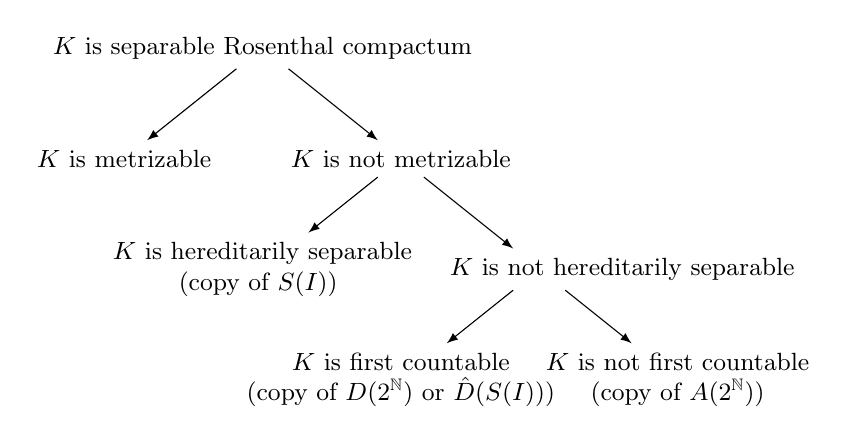
\begin{tikzpicture}[
  grow=down,
  sibling distance=10em,
  level distance=4em,
  edge from parent/.style={draw,-latex},
  every node/.style={font=\small,align=center}
  ]

\node {$K$ is separable Rosenthal compactum}
  child {node {$K$ is metrizable}
  }
  child {node {$K$ is not metrizable}
    child {node {$K$ is hereditarily separable \\ (copy of $S(I)$) \hspace{2cm}}}
    child {node {\hspace{2cm} $K$ is not hereditarily separable}
      child {node {$K$ is first countable \\ (copy of $D(2^\mathbb{N})$ or $\hat{D}(S(I))$)}}
      child {node {$K$ is not first countable \\ (copy of $A(2^\mathbb{N})$)}}
    }
  };

\end{tikzpicture}
\end{center}

The definitions provided here for NIP$_i$ ($i=1,2,3$) are topological.
This raises the following question:

\begin{question}
    Is there a non-topological characterization for NIP$_i$, $i=1,2,3$?
\end{question}


\subsection{The Argyros-Dodos-Kanellopoulos heptachotomy, and approximability of deep computation by minimal classes}

In the three separable cases given in \ref{E:Rosenthal comacta}, namely, $\hat{A}(2^\mathbb{N})$, $S(2^\mathbb{N})$ and $\hat{D}(S(2^\mathbb{N}))$, the countable dense subsets are indexed by the binary tree $2^{<\mathbb{N}}$.
This choice of index is useful for two reasons:
\begin{enumerate}
\item
Our emphasis is computational.
Elements of $2^{<\mathbb{N}}$ represent finite bitstrings, i.e.,  standard computations, while Rosenthal compacta represent deep computations, i.e., limits of finite computations.
Mathematically, deep computations are pointwise limits of standard computations.
However, computationally, we are interested in the manner (and the efficiency) in which the approximations can occur.
\item
Infinite branches of the binary tree $2^{<\mathbb{N}}$ correspond to the Cantor space $2^{\mathbb{N}}$, the canonical perfect set (in the sense that  any Polish space with no isolated points contains a copy of $2^{\mathbb{N}}$).
The use of infinite dimensional Ramsey theory for trees (pioneered by the work of James D. Halpern, Hans L\" auchli in \cite{halpern1966partition} and also Keith Milliken in \cite{milliken1981partition}, and Alain Louveau, Saharon Shelah, Boban Velickovic in \cite{louveau_shelah_velickovic_1993}) and perfect sets (Fred Galvin and Andreas Blass in \cite{Blass1981}, Arnold W. Miller in \cite{miller1989infinite}, and Stevo Todorcevic in \cite{Todorcevic_1999_CompactSubsetsBaire}) allowed S.A. Argyros, P. Dodos and V. Kanellopoulos in \cite{argyros2008rosenthal} to obtain an improved version of Theorem \ref{T:Todorcevic trichotomy}.
It is no surprise that Ramsey Theory becomes relevant in the study of Rosenthal compacta as it was a key ingredient in Rosenthal's $\ell_1$ Theorem.
For this reason, the main results in \cite{argyros2008rosenthal} (which we cite in this paper) are better explained by indexing Rosenthal compacta with the binary tree.
\end{enumerate}

\begin{defn}
Let $X$ be a Polish space.

\begin{enumerate}
\item
If  $I$ is a countable and $\{f_i:i\in I\}\subseteq\mathbb{R}^X$, $\{g_i:i\in I\}\subseteq\mathbb{R}^X$  are two pointwise families by  $I$, we say that $\{f_i:i\in\ I\}$ and $\{g_i:i\in I\}$ are \emph{equivalent} if and only if the map $f_i\mapsto g_i$ is extended to a homeomorphism from $\overline{\{f_i:i\in I\}}$ to $\overline{\{g_i:i\in I\}}$.
\item
If $\{f_t:t\in 2^{<\mathbb{N}}\}$ is a pointwise bounded family, we say that $\{f_t:t\in 2^{<\mathbb{N}}\}$ is \emph{minimal} if and only if for every dyadic subtree $\{s_t:t\in 2^{<\mathbb{N}}\}$ of $2^{<\mathbb{N}}$, $\{f_{s_t}:t\in 2^{<\mathbb{N}}\}$ is equivalent to $\{f_t:t\in 2^{<\mathbb{N}}\}$.
 \end{enumerate}
\end{defn}

One of the main results in \cite{argyros2008rosenthal} is that, up to equivalence,  there are  seven minimal families of Rosenthal compacta and that for every relatively compact $\{f_t:t\in 2^{<\mathbb{N}}\}\subseteq B_1(X)$ there is a dyadic subtree $\{s_t:t\in 2^{<\mathbb{N}}\}$ such that $\{f_{s_t}:t\in 2^{<\mathbb{N}}\}$ is equivalent to one of the minimal families.
We shall describe the seven minimal families next.
We follow the same notation as in \cite{argyros2008rosenthal}.
For any node $t\in 2^{<\mathbb{N}}$, let us denote by $t^\frown 0^{\infty}$ ($t^\frown 1^{\infty}$) the infinite binary sequence starting with $t$ and continuing will all $0$'s (respectively, all $1$'s).
Fix a regular dyadic subtree $R=\{s_t:t\in 2^{<\mathbb{N}}\}$ of $2^{<\mathbb{N}}$ (i.e., a dyadic subtree such that every level of $R$ is contained in a level of $2^{<\mathbb{N}}$) with the property that for all $s,s'\in R$, $s^\frown 0^{\infty}\neq s'^\frown 0^\infty$ and $s^\frown 1^{\infty}\neq s'^\frown 1^\infty$.
Given $t\in 2^{<\mathbb{N}}$, let $v_t$ be the characteristic function of the set $\{x\in 2^\mathbb{N}:x \text{ extends } t\}$.
Let $<$ be the lexicographic order in $2^\mathbb{N}$.
Given $a\in 2^{\mathbb{N}}$, let $f^+_a:2^{\mathbb{N}}\rightarrow\{0,1\}$ be the characteristic function of $\{x\in 2^{\mathbb{N}}:a\leq x\}$ and let $f^-_a:2^{\mathbb{N}}\rightarrow\{0,1\}$ be the characteristic function of $\{x\in 2^{\mathbb{N}}:a<x\}$.
Given two maps $f,g:2^{\mathbb{N}}\rightarrow\mathbb{R}$ we denote by $(f,g):2^{\mathbb{N}}\sqcup 2^{\mathbb{N}}\rightarrow\mathbb{R}$ the function which is $f$ on the first copy of $2^{\mathbb{N}}$ and $g$ on the second copy of $2^{\mathbb{N}}$.

\begin{enumerate}
    \item $D_1=\{\frac{1}{|t|+1}v_t:t\in 2^{<\mathbb{N}}\}$.
This is discrete in $\overline{D_1}=A(2^{\mathbb{N}})$.
    \item $D_2=\{s_t^\frown 0^{\infty}:t\in 2^{<\mathbb{N}}\}$.
This is discrete in $\overline{D_2}=2^{\leq N}$.
    \item $D_3=\{f^+_{s_t^\frown 0^\infty}:t\in 2^{<\mathbb{N}}\}$.
This is a discrete in $\overline{D_3}=S(2^{\mathbb{N}})$.
    \item $D_4=\{f^-_{s_t^\frown 1^\infty}:t\in 2^{<\mathbb{N}}\}$.
This is discrete in $\overline{D_4}=S(2^{\mathbb{N}})$.
    \item $D_5=\{v_t:t\in 2^{<\mathbb{N}}\}$.
This is discrete in $\overline{D_5}=\hat{A}(2^{\mathbb{N}})$.
    \item $D_6=\{(v_{s_t},s_t^\frown 0^\infty):t\in 2^{<\mathbb{N}}\}$.
This is discrete in $\overline{D_6}=\hat{D}(2^{\mathbb{N}})$.
    \item $D_7=\{(v_{s_t},x^+_{s_t^\frown 0^\infty}):t\in 2^{<\mathbb{N}}\}$.
This is discrete in $\overline{D_7}=\hat{D}(S(2^{\mathbb{N}}))$
\end{enumerate}

\begin{thm}[Heptachotomy of minimal families, Theorem 2 in \cite{argyros2008rosenthal}]
    Let $X$ be Polish.
For every relatively compact $\{f_{t}:t\in 2^{<\mathbb{N}}\}\subseteq B_1(X)$, there exists $i=1,2,\dots, 7$ and a regular dyadic subtree $\{s_t:t\in 2^{<\mathbb{N}}\}$ of $2^{<\mathbb{N}}$ such that $\{f_{s_t}:t\in 2^{<\mathbb{N}}\}$ is equivalent to $D_i$.
Moreover, all $D_i$ are minimal and mutually non-equivalent.
\end{thm}

\section{Measure-theoretic versions of NIP and universal Monte Carlo computability of  deep computations}
\label{Measure-theoretic NIP}

The countability assumption on $\mathcal{P}$  played a crucial  role in the proof of Theorem \ref{Generalized BFT} , as it makes $\mathbb{R}^\mathcal{P}$ a Polish space.
In this section, we do not assume that $\mathcal{P}$ is countable.
We replace deterministic computability by measure-theoretic (`Monte Carlo') computability.

\subsection{A measure-theoretic version of NIP}

The \emph{raison d'être} of the Baire class-1 functions is to work with a small class that contains the continuous functions and their pointwise limits, and that for perfectly normal $X$, a function  $f$ is in $B_1(X,Y)$ if and only if $f^{-1}[U]$ is an $F_\sigma$ subset of $X$ for every open $U\subseteq Y$ (see Fact~\ref{baire}).
This motivates the following definition:


\begin{defn}
\label{D:universal measurability}
Given a Hausdorff space $X$ and a measurable space $(Y,\Sigma)$, we say that $f:X\rightarrow Y$ is \emph{universally measurable} (with respect to $\Sigma$) if $f^{-1}(E)$ is $\mu$-measurable for every Radon measure%
\footnote{The definition Radon measure can be found in any standard measure theory textbook; see, for example, 411H in \cite{fremlin2003vol4}.
} $\mu$ on $X$ and every $E\in\Sigma$.
When $Y=\mathbb{R}$ we will always take $\Sigma=\mathcal{B}(\mathbb{R})$, the Borel $\sigma$-algebra of $\mathbb{R}$.
\end{defn}

\begin{rem} 
A function $f:X\rightarrow\mathbb{R}$ is universally measurable if and only if $f^{-1}(U)$ is $\mu$-measurable for every Radon probability measure $\mu$ on $X$ and every open set $U\subseteq\mathbb{R}$.

\end{rem}

Intuitively,  a function is universally measurable if it is ``measurable no matter which reasonable way you try to measure things on its domain".
The concept of universal measurability emerged from work of  Kallianpur and Sazonov, in the late 1950's and 1960s, with later developments by Blackwell, Darst, and others, building on earlier ideas of Gnedenko and Kolmogorov from the 1950s.
See~\cite[Chapters 1 and 2]{Pap:2002}.


\begin{notn}
Following \cite{BFT_1978_PCompactBaire}, the collection of all universally measurable real-valued functions on $X$ will be denoted by $M_r(X)$.
Given a fixed Radon measure $\mu$ on $X$, the collection of all $\mu$-measurable real-valued functions on $X$ will be denoted by $\mathscr{M}^0(X,\mu)$.
\end{notn}

In the context of deep computations, we will be interested in transition maps of a state space $L\subseteq \mathbb{R}^\mathcal{P}$ into itself.
There are two natural $\sigma$-algebras one can consider in the product space $\mathbb{R}^\mathcal{P}$: the Borel $\sigma$-algebra, i.e., the $\sigma$-algebra generated by open sets in $\mathbb{R}^\mathcal{P}$, and the cylinder $\sigma$-algebra (i.e., the $\sigma$-algebra generated by the sub-basic open sets in $\mathbb{R}^\mathcal{P}$, that is, the set $\pi_i^{-1}(U)$ with $U\subseteq \mathbb{R}$ open).
Note that when $\mathcal{P}$ is countable, both $\sigma$-algebras coincide, but in general the cylinder $\sigma$-algebra is strictly smaller.
We will use the cylinder $\sigma$-algebra to define universally measurable maps $f:\mathbb{R}^\mathcal{P}\rightarrow\mathbb{R}^\mathcal{P}$.
The reason for this choice is the following characterization:

\begin{prop}\label{prop:coordinated_univ_meas}
    Let $X$ be a Hausdorff space and $Y=\prod_{i\in I}Y_i$ be any product of measurable spaces $(Y_i,\Sigma_i)$ for $i\in I$.
Let $\Sigma_Y$ be the cylinder $\sigma$-algebra generated by the measurable spaces $(Y_i,\Sigma_i)$.
Let $f:X\rightarrow Y$.
The following are equivalent:
    \begin{enumerate}[(i)]
        \item
        $f:X\rightarrow Y$ is universally measurable (with respect to $\Sigma_Y$).
        \item
        $\pi_i\circ f:X\rightarrow Y_i$ is universally measurable (with respect to $\Sigma_i$) for all $i\in I$.
    \end{enumerate}
\end{prop}

\begin{proof}
    (i)$\Rightarrow$(ii) is clear since the projection maps $\pi_i$ are measurable and the composition of measurable functions is measurable.
To prove (ii)$\Rightarrow$(i), suppose that $C=\prod_{i\in I}C_i$ is a measurable cylinder and let $J$ be the finite subset of $I$ such that $C_i\neq Y_i$ for $i\in J$.
Then, $C=\bigcap_{i\in J}\pi_i^{-1}(C_i)$, so $f^{-1}(C)=\bigcap_{i\in J}(\pi_i\circ f)^{-1}(C_i)$ is a universally measurable set by assumption.
\end{proof}

The preceding proposition says that a transition map is universally measurable if and only if it is universally measurable on all its features; in other words, we can check measurability of a transition just by checking measurability feature by feature.
This is the same as in the Baire class-1 case (compare with lemma \ref{baire 1 and projections}).
We will denote by $M_r(X,\mathbb{R}^\mathcal{P})$ the collection of all universally measurable functions $f:X\rightarrow\mathbb{R}^\mathcal{P}$ (with respect to the cylinder $\sigma$-algebra), endowed with the topology of pointwise convergence.

In this paper we are interested in identifying PAC-learnability phenomena in real-valued deep computations (i.e., the NIP).
The main result in section \ref{S:Classification} is that PAC-learning (or NIP) corresponds to relative compactness in the space of Baire class-1 functions, whenever we work with countably many features.
The following measure-theoretic characterization of the NIP will lead us to find other connections between the topology of function spaces and a notion of Monte Carlo computability (see next section):

\begin{thm}[Bourgain-Fremlin-Talagrand, Theorem 2F in \cite{BFT_1978_PCompactBaire}]\label{BFT-2F}
    Let $X$ be a Hausdorff space and $A\subseteq C(X)$ be pointwise bounded.
The following are equivalent:
    \begin{enumerate}[(i)]
        \item
        $\overline{A}\subseteq M_r(X)$.
        \item 
        For every compact $K\subseteq X$, $A|_K$ satisfies the NIP.
        \item
        For every Radon measure $\mu$ on $X$, $A$ is relatively countably compact in $\mathscr{M}^0(X,\mu)$, i.e., every countable subset of $A$ has an accumulation point in $\mathscr{M}^0(X,\mu)$.
    \end{enumerate}
\end{thm}


\subsection{Universal Monte Carlo computability of  deep computations}

We now wish to define the concept of a deep computation being computable except on a set of arbitrarily small measure ``no matter which reasonable way you try to measure things on its domain"  (see the remarks following definition~\ref{D:universal measurability}).
This is the concept of \emph{universal Monte Carlo computability} defined below (Definition~\ref{D:universally essentially computable}).
To motivate the definition, we need to recall two facts:

\begin{enumerate}
\item
Littlewoood's second principle states that every Lebesgue measurable function is ``nearly continuous''.
The formal statement of this, which is Luzin's theorem, is that if
 $(X,\Sigma ,\mu )$  a Radon measure space and $Y$ is a second-countable topological space (e.g., $Y=\mathbb{R}^\mathcal{P}$ with $\mathcal{P}$ countable ) equipped with a Borel algebra, then any given $f:X\to Y$ is measurable if and only if for every  $E\in\Sigma$ and every $\varepsilon>0$ there exists a closed $F\subseteq E$ such that the restriction $f|_F$ is continuous and $\mu(E\backslash F) < \varepsilon$.
\item
Computability of deep computations is characterized in terms of continuous extendibility of computations.
This is at the core of~\cite{alva2024approximability}.
\end{enumerate}


These two facts motivate the following definition:


\begin{defn}
\label{D:universally essentially computable}
    Let $(L,\mathcal{P},\Gamma)$ be a CCS.
We say that a transition $f:L\rightarrow L$ is \emph{universally Monte Carlo computable} if and only if there exists $\tilde f:\mathcal{L}_{\text{sh}}\rightarrow \mathcal{L}_{\text{sh}}$ extending $f$ such that for every sizer $r_\bullet$ there is a sizer $s_\bullet$ such that the restriction $\tilde f|_{\mathcal{L}[r_{\bullet}]}:\mathcal{L}[r_\bullet]\rightarrow\mathcal{L}[s_\bullet]$ is universally measurable, i.e., $\pi_P\circ \tilde f|_{\mathcal{L}[r_{\bullet}]}:\mathcal{L}[r_\bullet]\rightarrow [-s_P,s_P]$ is $\mu$-measurable for every Radon probability measure $\mu$ on $\mathcal{L}[r_\bullet]$ and $P\in\mathcal{P}$.
\end{defn}

\begin{rem}
    Recall that every Radon measure on a compact space (e.g., $\mathcal{L}_{\text{sh}}$) is finite and, by proper normalization, can be treated as probability measures.
    For this reason we use the term ``Radon probability measure'' instead of ``Radon measure'' in definition \ref{D:universally essentially computable}.
\end{rem}

\subsection{Bourgain-Fremlin-Talagrand, NIP, and universal Monte Carlo computability of  deep computations}

The result in this subsection is a consequence of Theorem~\ref{BFT-2F}.
It says that PAC-learning (or NIP) implies Monte Carlo computability with respect to any measure.

\begin{thm}\label{T:NIP and Monte Carlo}
    Let $(L,\mathcal{P},\Gamma)$ be a CCS satisfying the Extendibility Axiom.
Let $R$ be an exhaustive collection of sizers.
Let $\Delta\subseteq\Gamma$ be $R$-confined.
If $\pi_P\circ\Delta|_{L[r_\bullet]}$ satisfies the NIP for all $P\in\mathcal{P}$ and all $r_{\bullet}\in R$, then every deep computation in $\Delta$ is universally Monte Carlo computable.
\end{thm}

\begin{proof}
    Fix $P\in\mathcal{P}$ and $r_\bullet\in R$.
    By the Extendibility Axiom, $\pi_P\circ\tilde\Delta|_{\mathcal{L}[r_\bullet]}$ is a set of pointwise bounded continuous functions on the compact set $\mathcal{L}[r_\bullet]$.
    Since $\pi_P\circ\tilde\Delta|_{L[r_\bullet]}=\pi_P\circ\Delta|_{L[r_\bullet]}$ has the NIP then so does $\pi_P\circ\tilde\Delta|_{\mathcal{L}[r_\bullet]}$ by lemma \ref{NIP and closure}.
    By Theorem \ref{BFT-2F}, we have $\overline{\pi_P\circ\tilde\Delta|_{\mathcal{L}[r_\bullet]}}\subseteq M_r(\mathcal{L}[r_\bullet])$ for all $r_\bullet\in R$ and $P\in\mathcal{P}$.
    Let $f\in\overline{\Delta}$ be a deep computation.
    Write $f=\mathcal{U}\lim_i\gamma_i$ as an ultralimit of computations in $\Delta$.
    Define $\tilde{f}:=\mathcal{U}\lim_i\tilde{\gamma_i}$.
    Then, $\tilde{f}:\mathcal{L}_{\text{sh}}\rightarrow \mathcal{L}_{\text{sh}}$ extends $f$.
    Since $\Delta$ is $R$-confined we have that $f:L[r_\bullet]\rightarrow L[r_\bullet]$ and $\tilde{f}:\mathcal{L}[r_\bullet]\rightarrow \mathcal{L}[r_\bullet]$ for all $r_\bullet\in R$.
    Lastly, note that for all $r_\bullet\in R$ and $P\in\mathcal{P}$ we have that $\pi_P \circ \tilde{f}|_{\mathcal{L}[r_\bullet]}\in \overline{\pi_P\circ\tilde\Delta|_{\mathcal{L}[r_\bullet]}}\subseteq M_r(\mathcal{L}[r_\bullet])$.
\end{proof}

\begin{question}
Under the same assumptions of the preceding theorem, suppose that every deep computation of $\Delta$ is universally Monte Carlo computable.
Must $\pi_P\circ\Delta|_{L[r_\bullet]}$ have the NIP for all $P\in\mathcal{P}$ and all $r_{\bullet}\in R$?
\end{question}

\subsection{Talagrand stability, Fremlin's dichotomy, NIP, and universal Monte Carlo computability of  deep computations}

There is another notion closely related to NIP, introduced by Talagrand in \cite{talagrand1984pettis} while studying Pettis integration.
Suppose that $X$ is a compact Hausdorff space and $A\subseteq \mathbb{R}^X$.
Let $\mu$ be a Radon probability measure on $X$.
Given a $\mu$-measurable set $E\subseteq X$, a positive integer $k$ and real numbers $a<b$.
we write:

$$D_k(A,E,a,b)=\bigcup_{f\in A}\{x\in E^{2k}:f(x_{2i})\leq a, \hspace{1mm} f(x_{2i+1})\geq b \hspace{1mm}{\text{ for all }i<k} \}$$

We say that $A$ is \emph{Talagrand $\mu$-stable} if and only if for every $\mu$-measurable set $E\subseteq X$ of positive measure and for every $a<b$ there is $k\geq 1$ such that
\[
(\mu^{2k})^*(D_k(A,E,a,b))<(\mu(E))^{2k},
\]
where $\mu^*$ denotes the outer measure (we work with outer since the sets $D_k(A,E,a,b)$ need not be $\mu$-measurable).
This is certainly the case when $A$ is a countable set of continuous (or $\mu$-measurable) functions.

We shall now establish that Talagrand $\mu$-stability is a way to ensure that accumulation points (deep computations) are $\mu$-measurable.
First, we mention the following useful characterization of measurable functions (compare with Fact \ref{baire}):

\begin{fact}[Lemma 413G in \cite{fremlin2003vol4}]\label{fact: measurable functions characterization}
    Suppose that $(X,\Sigma,\mu)$ is a measure space and $\mathcal{K}\subseteq\Sigma$ is a collection of measurable sets satisfying the following conditions:
    \begin{enumerate}
        \item $(X,\Sigma,\mu)$ is complete, i.e., for all $E\in\Sigma$ with $\mu(E)=0$ and $F\subseteq E$ we have $F\in\Sigma$.
        \item $(X,\Sigma,\mu)$ is semi-finite, i.e., for all $E\in\Sigma$ with $\mu(E)=\infty$ there exists $F\subseteq E$ such that $F\in\Sigma$ and $0<\mu(F)<\infty$.
        \item $(X,\Sigma,\mu)$ is saturated, i.e., $E\in\Sigma$ if and only if $E\cap F\in\Sigma$ for all $F\in\Sigma$ with $\mu(F)<\infty$.
        \item $(X,\Sigma,\mu)$ is inner regular with respect to $\mathcal{K}$, i.e., for all $E\in\Sigma$
        $$\mu(E)=\sup\{\mu(K):K\in\mathcal{K} \text{ and } K\subseteq E\}$$
    \end{enumerate}
    (In particular, if $X$ is Hausdorff, $\mu$ is a Radon measure on $X$ and $\mathcal{K}$ is the collection of compact subsets of $X$, all these conditions hold).
    Then, $f:X\rightarrow\mathbb{R}$ is measurable if and only if for every $K\in\mathcal{K}$ with $0<\mu(K)<\infty$ and $a<b$, either $\mu^*(P)<\mu(K)$ or $\mu^*(Q)<\mu(K)$ where $P=\{x\in K:f(x)\leq a\}$ and $Q=\{x\in K:f(x)\geq b\}$.
\end{fact}

\begin{lem}\label{talagrand stable is relatively compact}
    If $A$ is Talagrand $\mu$-stable, then $\overline{A}$ is also Talagrand $\mu$-stable and $\overline{A}\subseteq\mathscr{M}^0(X,\mu)$.
\end{lem}

\begin{proof}
    First, we claim that a subset of a $\mu$-stable set is $\mu$-stable.
    To see this, suppose that $A\subseteq B$ and $B$ is $\mu$-stable.
    Fix any $\mu$-measurable $E\subseteq X$ of positive measure and $a<b$.
    Let $k\geq 1$ such that
    \[
    (\mu^{2k})^*(D_k(B,E,a,b))<(\mu(E))^{2k}
    \]
    Since $A\subseteq B$, then $D_k(A,E,a,b)\subseteq D_k(B,E,a,b)$ so
    \[
    (\mu^{2k})^*(D_k(A,E,a,b))\leq (\mu^{2k})^*(D_k(B,E,a,b))<(\mu(E))^{2k}
    \]
    We now show that $\overline{A}$ is $\mu$-stable.
    Fix $E\subseteq X$ measurable with positive measure and $a<b$.
    Let $a'<b'$ be such that $a<a'<b'<b$.
    Since $A$ is $\mu$-stable, let $k\geq 1$ be such that
    \[
    (\mu^{2k})^*(D_k(A,E,a',b'))<(\mu(E))^{2k}
    \]
    If $x\in D_k(\overline{A},E,a,b)$, then there is $f\in\overline{A}$ such that $f(x_{2i})\leq a<a'$ and $f(x_{2i+1})\geq b>b'$ for all $i<k$.
    By definition of pointwise convergence topology, there exists $g\in A$ such that $g(x_{2i})<a'$ and $g(x_{2i+1})>b'$ for all $i<k$.
    Hence, $x\in D_k(A,E,a',b')$.
    We have shown that $D_k(\overline{A},E,a,b)\subseteq D_k(A,E,a',b')$ so
    \[
    (\mu^{2k})^*(D_k(\overline{A},E,a,b))\leq (\mu^{2k})^*(D_k(A,E,a',b'))<(\mu(E))^{2k}
    \]
    It suffices to show that $\overline{A}\subseteq \mathscr{M}^0(X,\mu)$.
    Suppose that there exists $f\in\overline{A}$ such that $f\notin \mathscr{M}^0(X,\mu)$.
    By fact \ref{fact: measurable functions characterization}, there exists a $\mu$-measurable set $E$ of positive measure and $a<b$ such that $\mu^*(P)=\mu^*(Q)=\mu(E)$ where $P=\{x\in E: f(x)\leq a\}$ and $Q=\{x\in E: f(x)\geq b\}$.
    Then, for any $k\geq 1$: $(P\times Q)^k\subseteq D_k(\{f\},E,a,b)$ so $(\mu^{2k})^*(D_k(\{f\},E,a,b))=(\mu^*(P)\mu^*(Q))^k=(\mu(E))^{2k}$.
    Thus, $\{f\}$ is not $\mu$-stable, but we argued before that a subset of a $\mu$-stable set must be $\mu$-stable.
    Contradiction.
\end{proof}

Just like the NIP, Talagrand $\mu$-stability is directly related to relative compactness in the space $\mathscr{M}^0(X,\mu)$.
This is the content of the preceeding lemma.

\begin{defn}
We say that $A$ is \emph{universally Talagrand stable} if $A$ is Talagrand $\mu$-stable for every Radon probability measure $\mu$ on $X$.
\end{defn}

We first observe  that universal Talagrand stability corresponds to a complexity class smaller than or equal to the NIP;
in other words, that every universally Talagrand stable set satisfies the NIP:

\begin{prop}\label{prop:Talagrand implies NIP}
    Let $X$ be a compact Hausdorff space and $A\subseteq C(X)$ be pointwise bounded.
If $A$ is universally Talagrand stable, then $A$ satisfies the NIP.
\end{prop}

\begin{proof}
    By Theorem \ref{BFT-2F}, it suffices to show that $A$ is relatively countably compact in $\mathscr{M}^0(X,\mu)$ for all Radon probability measure $\mu$ on $X$.
Since $A$ is Talagrand $\mu$-stable for any such $\mu$, we have $\overline{A}\subseteq\mathscr{M}^0(X,\mu)$ by lemma \ref{talagrand stable is relatively compact}.
In particular, $A$ is relatively countably compact in $\mathscr{M}^0(X,\mu)$.
\end{proof}

In the computational context we get the following:

\begin{cor}\label{T:Talagrand stability and Monte Carlo}
    Let $(L,\mathcal{P},\Gamma)$ be a CCS satisfying the Extendibility Axiom.
If $\pi_P\circ\Delta|_{L[r_\bullet]}$ is universally Talagrand stable for all $P\in\mathcal{P}$ and all sizers $r_{\bullet}$, then every deep computation is universally Monte Carlo computable.
\end{cor}

\begin{proof}
    This is a consequence of proposition \ref{prop:Talagrand implies NIP} and Theorem 4.8.
\end{proof}

In the measure-theoretic side, we have identified two notions of PAC-learnability: Talagrand stability with respect to any measure and the NIP, which can also be described in measure-theoretic terms. 
A natural question is whether these two classes are equivalent. 
Even in the simple case of countably many computations, this question is sensitive to the set-theoretic axioms. 
On one hand, it is consistent (with respect to the standard ZFC axioms of set theory) that these two classes are the same:

\begin{thm}[Talagrand, Theorem 9-3-1(a) in \cite{talagrand1984pettis}]
    Let $X$ be a compact Hausdorff space and $A\subseteq M_r(X)$ be countable and pointwise bounded.
Assume that $[0,1]$ is not the union of $<\mathfrak{c}$ closed measure zero sets.
If $A$ satisfies the NIP, then $A$ is universally Talagrand stable.
\end{thm}

The assumption that $[0,1]$ is not the union of $<\mathfrak{c}$ closed measure zero sets is a consequence of, for example, the Continuum Hypothesis.
On the other hand, by fixing a particular well-known measure: the Lebesgue measure, we see that the other case is also consistent:

\begin{thm}[Fremlin, Shelah, \cite{fremlin1993pointwise}]
    It is consistent with the usual axioms of set theory that there exists a countable pointwise bounded set of Lebesgue measurable functions with the NIP which is not Talagrand stable with respect to Lebesgue measure.
\end{thm}

Notice that in the framework presented in this paper, we are interested in continuous computations and their limits. 
The previous two results apply to sets of measurable functions, a higher level of computability than continuity.
It is possible that the continuity assumption, i.e., the Extendibility Axiom, settles the problem. 
This is a problem that remains open for future work.


\begin{comment}

\section*{Appendix: Measure Theory}

Given a set $X$, a collection $\Sigma$ of subsets of $X$ is called a \emph{$\sigma$-algebra} if $\Sigma$ contains $X$ and is closed under complements and countable unions.
Hence, for example, a $\sigma$-algebra is also closed under countable intersections.
Intuitively, a $\sigma$-algebra is a collection of sets in which we can define a $\sigma$-additive measure.
We call sets in a $\sigma$-algebra $\Sigma$ \emph{measurable sets} and the pair $(X,\Sigma)$ a measurable space.
If $X$ is a topological space, there is a natural $\sigma$-algebra of subsets of $X$, namely the \emph{Borel $\sigma$-algebra} $\mathcal{B}(X)$, i.e., the smallest $\sigma$-algebra containing all open subsets of $X$.
Given two measurable spaces $(X,\Sigma_X)$ and $(Y,\Sigma_Y)$, we say that a function $f:X\rightarrow Y$ is \emph{measurable} if and only if $f^{-1}(E)\in\Sigma_X$ for every $E\in \Sigma_Y$.
In particular, we say that $f:X\rightarrow\mathbb{R}$ is measurable if $f^{-1}(E)\in \Sigma_X$ for all $E\in\mathcal{B}(\mathbb{R})$ (equivalently, $E$ open in $\mathbb{R}$).

Given a measurable space $(X,\Sigma)$, a \emph{$\sigma$-additive measure} is a non-negative function $\mu:\Sigma\rightarrow\mathbb{R}$ with the property that $\mu(\emptyset)=0$ and $\mu(\bigcup_{n=0}^\infty A_n)=\sum_{n=0}^\infty\mu(A_n)$ whenever $\{A_n:n\in\mathbb{N}\}\subseteq\Sigma$ is pairwise disjoint.
We call $(X,\Sigma,\mu)$ a \emph{measure space}.
A $\sigma$-additive measure is called a \emph{probability measure} if $\mu(X)=1$.
A measure $\mu$ is \emph{complete} if for every $A\subseteq B\in\Sigma$, $\mu(B)=0$ implies $A\in\Sigma$.
In words, subsets of measure-zero sets are always measurable (and hence, by the monotonicity of $\mu$, have measure zero as well).
A measure $\mu$ is \emph{$\sigma$-finite} if $X=\cup_{n=1}^\infty X_n$ where $\mu(X_n)<\infty$ for all $n\in\mathbb{N}$ (i.e., $X$ can be decomposed into countably many finite measure sets).
A measure $\mu$ is \emph{perfect} if for every measurable $f:X\rightarrow\mathbb{R}$ and every measurable set $E$ with $\mu(E)>0$, there exists a compact $K\subseteq f(E)$ such that $\mu(f^{-1}(K))>0$.
We say that a property $\phi(x)$ about $x\in X$ holds \emph{$\mu$-almost everywhere} if $\mu(\{x\in X:\varphi(x) \text{ does not hold}\})=0$.

A special example of the preceding concepts is that of a \emph{Radon measure}.
If $X$ is a Hausdorff topological space, then a measure $\mu$ on the Borel sets of $X$ is called a \emph{Radon measure} if
\begin{itemize}
    \item for every open set $U$, $\mu(U)$ is the supremum of $\mu(K)$ over all compact $K\subseteq U$, that is, the measure of open sets may be approximated via compact sets; and
    \item every point of $X$ has a neighborhood $U\ni x$ for which $\mu(U)$ is finite.
\end{itemize}

The most famous nontrivial example of a Radon measure on $\mathbb{R}$ is the Lebesgue measure of Borel sets.
If $X$ is finite, $\mu(A):=|A|$ (the cardinality of $A$) defines a Radon measure on $X$.
Every Radon measure is perfect (see 451A, 451B and 451C in \cite{fremlin2003vol4}).

While not immediately obvious, sets can be measurable according to one measure, but non-measurable according to another.
Given a measure space $(X,\Sigma,\mu)$ we say that a set $E\subseteq X$ is \emph{$\mu$-measurable} if there are $A,B\in \Sigma$ such that $A\subseteq E\subseteq B$ and $\mu(B\backslash A)=0$.
The set of all $\mu$-measurable sets is a $\sigma$-algebra containing $\Sigma$ and it is denoted by $\Sigma_\mu$.
A set $E\subseteq X$ is \emph{universally measurable} if it is $\mu$-measurable for every Radon probability measure on $X$.
It follows that Borel sets are universally measurable.
We say that $f:X\rightarrow\mathbb{R}$ is \textit{$\mu$-measurable} if $f^{-1}(E)\in\Sigma_\mu$ for all $E\in\mathcal{B}(\mathbb{R})$ (equivalently, $E$ open in $\mathbb{R}$).


Recall that if $\{X_i:i\in I\}$ is a collection of topological spaces indexed by some set $I$, then the product space $X:=\prod_{i\in I}X_i$ is endowed with the topology generated by \emph{cylinders}, that is, sets of the form $\prod_{i\in I} U_i$ where each $U_i$ is open in $X_i$, and $U_i=X_i$ except for finitely many indices $i\in I$.
If each space is measurable, say we pair $X_i$ with a $\sigma$-algebra $\Sigma_i$, then there are multiple ways to interpret the product space $X$ as a measurable space, but the interpretation we care about in this paper is the so called \emph{cylinder $\sigma$-algebra}, as used in Lemma~\ref{lemma:coordinated_univ_meas}.
Namely, let $\Sigma$ be the $\sigma$-algebra generated by sets of the form $$\prod_{i\in I}C_i,\quad C_i\in\Sigma_i,\ C_i=X_i\ \text{for all but finitely many }i\in I.$$

We remark that when $I$ is uncountable and $\Sigma_i=\mathcal{B}(X_i)$ for all $i\in I$, then $\Sigma$ is, in general, strictly \textbf{smaller} than $\mathcal{B}(X)$.


\end{comment}

%%%%%%%%%%%%%%%%%%%%%%%%%%%%%%%%%%%%%%%%%%%%%%%%%%%%%%%%%%%%%%%%%%%%%%%%%%



%%%%%%%%%%%%%%%%%%%%%%%%%%%%%%%%%%%%%%%%%%%%%%%%%%%%%%%%%%%%%%%%%

%\begin{thebibliography}{9}



\bibliographystyle{alpha}
\nocite{*}
\bibliography{bib}

%\end{thebibliography}
\end{document}
